\documentclass[9pt,twocolumn,twoside,lineno]{pnas-new}

% Use the lineno option to display guide line numbers if required.

% packages
\usepackage{courier}
\usepackage{multirow}

\templatetype{pnasresearcharticle} % Choose template 
% {pnasresearcharticle} = Template for a two-column research article
% {pnasmathematics} %= Template for a one-column mathematics article
% {pnasinvited} %= Template for a PNAS invited submission

\title{Genomic architecture controls multivariate adaptation to climate change}

% Use letters for affiliations, numbers to show equal authorship (if applicable) and to indicate the corresponding author
\author[a,1]{Drew E. Terasaki Hart}
\author[a]{Ian J. Wang}

\affil[a]{Department of Environmental Science, Policy, and Management, University of California, Berkeley, CA 94720}

% Please give the surname of the lead author for the running footer
\leadauthor{Terasaki Hart} 

% Please include corresponding author, author contribution and author declaration information
\authorcontributions{D.E.T.H. conceived, designed and wrote the simulations and analysis, and wrote the manuscript. I.J.W. helped conceive and design the simulations and analysis, and cowrote the manuscript.}
\authordeclaration{The authors declare no competing interests.}
\correspondingauthor{\textsuperscript{1}To whom correspondence should be addressed. E-mail: drew.hart@berkeley.edu}

% At least three keywords are required at submission. Please provide three to five keywords, separated by the pipe symbol.
\keywords{adaptation $|$ climate change $|$ $|$ landscape genomics $|$ spatial simulation $|$ gene flow $|$ genetic architecture} 

\begin{abstract}
% NOTE: 250 WORDS MAX!
% NOTE: THIS NEEDS REFINING AND SHORTENING; THREW TOGETHER IN 10 MINUTES
As climate change advances,
environmental gradients will frequently decouple,
leading to the emergence of novel multivariate 
environments that will exert increasing stress on wild populations.
Evolutionary responses are expected to be one of the main ways in which
populations may adjust and survive,
with a common expectation
that local adaptation may occur by way of up-gradient gene flow
that brings adaptive diversity 
into populations whose future climates are well
approximated by the current climate of source populations.
However, multivariate selective environments in the real world can have
profound evolutionary importance,
potentially generating dynamics that complicate that simplified model
--- yet, they have been largely overlooked in most
research on climate change adaptation so far.
The genomic architecture of climate-adapted traits
may also exert major influence on evolutionary dynamics
under climate change, and hence on long-term conservation outcomes,
but is poorly understood and expected to be vary widely across taxa.
Here, we use \textit{geonomics}, a Python package
for constructing landscape genomic simulations
on complex and changing landscapes,
to simulate multivariate evolutionary responses to climate change
under various genomic architectures --- combinations of polygenicity, genotypic redundancy,
and linkage between loci underlying adaptive traits.
We use the results to test a series of hypotheses about microevolutionary responses to climate change.
While we corroborate some theoretical results reported from previous models
based on univariate or static environments,
our results also extend and complicate established theory in a few ways.
First, while we find that up-gradient gene flow under climate change is always at least
equal to or greater than that in null models, it is strongly constrained
under lower linkage and higher polygenicity, suggesting that \textit{in situ} shifts
in allelic covariance may be a more effective mechanism of adaptation
under some conditions.
Second, we find that stronger linkage and higher polygenicity also
decrease adaptive capacity, increase maladaptation, and thus exacerbate
demographic declines under climate change, even leading to failure to
adapt and local extinction in the most extreme circumstances.
Finally, we find that adaptive capacity increases under 
higher genotypic redundancy across all scenarios,
contributing to the growing
recognition of redundancy as an important facet of genomic
architecture and suggesting directions for better understanding
and predicting the climatic vulnerability of real populations.
\end{abstract}


% Please add a significance statement to explain the relevance of your work
\significancestatement{Authors must submit a 120-word maximum statement about the significance of their research paper written at a level understandable to an undergraduate educated scientist outside their field of speciality. The primary goal of the significance statement is to explain the relevance of the work in broad context to a broad readership. The significance statement appears in the paper itself and is required for all research papers.}

\dates{This manuscript was compiled on \today}
\doi{\url{www.pnas.org/cgi/doi/10.1073/pnas.XXXXXXXXXX}}

\begin{document}

\maketitle
\thispagestyle{firststyle}
\ifthenelse{\boolean{shortarticle}}{\ifthenelse{\boolean{singlecolumn}}{\abscontentformatted}{\abscontent}}{}


\dropcap{C}limate change is one of the foremost threats to biodiversity in the Anthropocene.
The ability of species to persist within their current ranges will likely depend largely upon their abilities to
locally adapt to climate change through natural selection - a concept frequently referred to 
as `adaptive capacity’ or `evolutionary potential’ (\cite{chevin,harrisson,nicotra,vilas,wade}).
Because adaptive \textit{de novo} mutations take a long time to arise,
this adaptation will instead most likely be facilitated
by the reconfiguration of existing adaptive diversity \cite{bomblies}.
A common conceptual model underlying this assumption is that of
adaptive gene flow parallel to a shifting climatic gradient
(i.e., in the vector
direction of climate velocity; \cite{ackerly}),
which would bring beneficial genes into recipient populations
from 'climate-suitable' populations --- i.e., populations whose
current climates approximate future local projections \cite{bellis}.
This model of adaptive gene flow has both theoretical
\cite{aitken_whitlock,slatkin,tigano}
and empirical 
\cite{feder,bell}
support
but meets resistance under theoretical conditions in which gene flow can be maladaptive
\cite{wang,lenormand,slatkin,haldane,wright,felsenstein}.
In these circumstances, shifting allelic covariance --- 
 the \textit{in situ} recombination of standing genetic variation into new,
adaptive genotypes --- could be a more efficient mechanism of local adaptation to environmental change.

In recent decades, research bridging the fields
of molecular population genetics
and quantitative genetics
\cite{barghi_polygenic,barton,pritchard_human_adaptation,pritchard_sweeps_alone}
has revealed that the genetic architecture of a trait
is a core determinant of whether and how that trait
becomes locally adapted \cite{yeaman_review}.
The number of loci underlying a trait (henceforth, 'polygenicity'),
the rate of recombination between trait loci (i.e., linkage),
and the number of distinct genotypes that yield identical trait phenotypes
(i.e., genotypic redundancy; \cite{yeaman_review,laruson,barghi_polygenic})
are among the key aspects of genetic architecture that influence adaptation
\cite{barton,yeaman_whitlock,yeaman_review,lecorre}.
Previous research suggests that ecologically-important traits can vary from
few loci of large effect \cite{martin,rees}
to many loci of small effect \cite{boyle,rockman,savolainen,sella,barghi_polygenic},
and shows that this variation in polygenicity can
determine the rate and nature of local adaptation \cite{yeaman_amnat}. 
Linkage controls the likelihood that adaptive alleles cluster together,
essentially forming alleles of larger effect size that are stronger 
targets of selection and more resistant
to swamping gene flow \cite{yeaman_whitlock},
thereby facilitating local adaptation \cite{tigano}.
Genotypic redundancy can facilitate local adaptation 
by allowing the existence of a stable phenotypic cline
subtended by a genotypic dynamic equilibrium
consisting of continuous and concerted shifts in non-neutral allele frequencies
(i.e., 'transient genetic architectures' \cite{barghi_redundancy,manceau,yeaman_amnat}).

The influence of genetic architecture on the nature and outcomes
of local adaptation to changing environmental gradients
has been studied to a limited extent,
with nearly exclusive focus on univariate models
of the selective environment (but see \cite{schiffers}).
Yet, such models have limitations for studying adaptation to climate change
because species can be simultaneously adapted to multiple,
unaligned environmental gradients \cite{guillaume} that can shift differentially
and thus decouple as climate change advances
\cite{crimmins,daly},
leading to the emergence of novel multivariate landscapes
\cite{williams_novel_climates,williams_projected_novel_disappearing,fitzpatrick_climate_novelty_forecasts}.
Under these circumstances,
gene flow from 'climate-suitable' populations
may not be universally adaptive
if the incoming haplotypes conferring
a fitness advantage for a climate-adapted trait
also contain genetic variation that could cause conflicting
fitness effects for other traits adapted to non-climatic and decoupling gradients,
such that the evolutionary outcome could depend on
the genetic architectures of the traits involved
\cite{aitken_whitlock,schiffers}.
The genomic architecture of locally adapted traits
can influence the relative magnitudes of the maladaptation resulting from gene flow
and that resulting from shifting allelic covariance \textit{in situ},
and can thus determine the relative contributions of these two processes to
 adaptation under climate change --- or, indeed,
whether adaptation occurs at all.

Spatially explicit simulation is one of our strongest tools
for improving our understanding of the complex dynamics of gene flow and adaptation
under climate change \cite{capblancq_review}.
In this study, we use individual-based, spatially explicit simulations
to test how genetic architecture influences multivariate adaptation to climate change.
We first simulate 
the adaptation of a population to a bivariate environment composed of two horizontal 
environmental gradients, each exerting selection on a separate trait.
In our main models, we then simulate climate change on that landscape by holding one gradient 
constant while gradually shifting the other gradient horizontally, such that
the decoupling environment pushes local fitness peaks toward novel regions 
of bivariate trait space (Fig. \ref{fig:conceptual}).
We run 100 pairs of climate change
and null (i.e., stable climate) simulations, for each of eighteen scenarios
resulting from the full factorial crossing of three key components
of genomic architecture: genotypic redundancy, polygenicity, and linkage
(the precise values of which are given in Table \ref{tab:tab_1}).

\begin{table}
\begin{tabular}{b{0.35\linewidth}b{0.05\linewidth}b{0.45\linewidth}}
\hline
\textbf{component} & \textbf{level} & \textbf{parameter value} \\
\hline
\multirow{2}{10em}{genotypic redundancy} \\
& low: & $\texttt{redund}=1$ \\
& high: & $\texttt{redund}=2$ \\
\hline
\multirow{3}{10em}{polygenicity} \\
& low: & $\texttt{n\_loci}=4\times \texttt{redund}$ \\ 
& mod: & $\texttt{n\_loci}=20\times \texttt{redund}$ \\
& high: & $\texttt{n\_loci}=100\times \texttt{redund}$ \\
\hline
\multirow{3}{10em}{linkage} \\
& low: & $\texttt{recomb}=0.5$ \\
& mod: & $\texttt{recomb}=0.05$ \\
& high: & $\texttt{recomb}=0.005$ \\
\hline
\end{tabular}
\medskip
\caption{\label{tab:tab_1}Parameter values used for each of the three focal components of genomic architecture parameters. The full factorial combinations of these parameter values constitute the set of 18 simulation scenarios for which we present results. Of note, the interaction between the \texttt{n\_loci} and \texttt{redund} parameter values creates, in low-redundancy scenarios, genotype-phenotype mappings that are many-to-one for intermediate phenotypes but decline to one-to-one mappings at extreme phenotypes, but creates, in high-redundancy scenarios, many-to-one mappings across all phenotypes between 0 and 1, inclusive --- i.e., across all phenotypes that are optimal within environmental values occurring somewhere on the landscape.}
\end{table}

\begin{figure}%[tbhp]
\centering
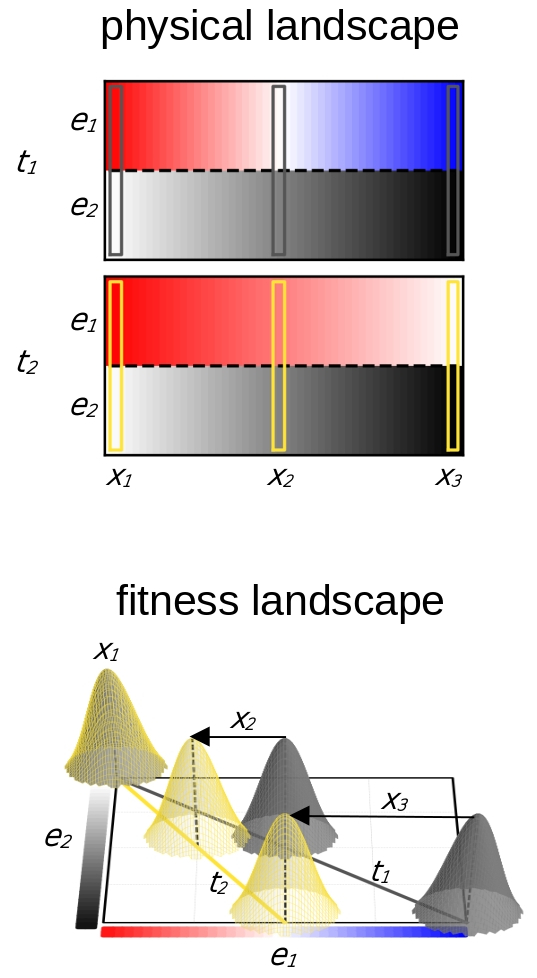
\includegraphics[width=.8\linewidth]{pub/figs/FIG_1_conceptual.jpg}
    \caption{Conceptual model of adaptation to climate change. Above: Stacked, horizontal cross-sections of our square simulation landscape, shown for the shifting environmental gradient ($e_{1}$, blue-red color ramp) and the stable gradient ($e_{2}$, white-black color ramp), both before climate change ($t_{1}$) and after ($t_{2}$). Below: Bivariate fitness landscape of the traits adapted to the shifting and stable gradients, on axes $e_{1}$ and $e_{2}$, respectively. Three example positions along the bivariate gradient ($x_{1}$, $x_{2}$, $x_{3}$) are delineated by thin vertical boxes on the physical landscape, both before climate change (gray) and after (yellow), and their corresponding fitness peaks are shown as color-matched kernels located along color-matched lines of the fitness optima that exist on the physical landscape before ($t_{1}$) and after ($t_{2}$) climate change. Shifts in local fitness peaks are shown as labeled arrows ($x_{2}$, $x_{3}$); the environment at the far left of the physical landscape does not change, so $x_{1}$'s fitness peaks are overlapping and have no shift, whereas the environment at the far right of the physical landscape experiences the maximal rate of change, which is reflected in the shift in $x_{3}$'s fitness peaks. Note that fitness peaks are stylized and truncated for ease of depiction; in our simulations, fitness decreases as a linear function of an individual's distance from its phenotypic optimum, rather than the truncated Gaussian function depicted here.}
\label{fig:fig_1}
\end{figure}


We use our simulations to test a series of hypotheses about the influence of genomic architecture 
on multivariate adaptation under climate change. First, we hypothesize that up-gradient 
gene flow will be higher under climate change than under a stable climate across all
scenarios but that gene flow contributes least to climate change adaptation when
linkage is low and polygenicity is high.
This is because we expect gene flow to always have
at least some adaptive value, but we also expect low-linkage, high-polygenicity architectures 
(i.e., 'dispersed' architectures \cite{yeaman_review}) to exhibit quick \textit{in situ}
adaptation by way of shifting allelic covariance among many small-effect alleles, akin to adaptation 
under transient genetic architectures, facilitating phenotypic shifts in the absence of up-gradient gene flow.
Second, we hypothesize that stronger linkage 
and higher polygenicity will reduce a population's adaptive capacity under climate change,
manifesting as greater reductions in population size and mean fitness
and more persistent maladaptation, because both conditions impose longer expected
wait times for the emergence of recombinant haplotypes that push phenotypes
away from their pre-change fitness peaks. Finally, we hypothesize that higher genotypic redundancy
facilitates adaptation to shifting gradients, much as it does on stable gradients 
\cite{barghi_redundancy,manceau,yeaman_amnat}, resulting in smaller reductions 
in population size and mean fitness.




\section*{Results}

\subsection{Gene flow}
Climate change led to a nearly universal increase in up-gradient gene flow
compared to null simulations: difference in gene flow was $>0$ in all scenarios
in Fig. \ref{fig:fig_2}, and in our regression
results the fitted values' 95\% confidence intervals were $>0$ in all but
one (the moderate-polygenicity, low-linkage, high-redundancy secenario, where the confidence interval was just below 0).
However, the magnitude of this increase was minimal under
some scenarios, and was positively correlated with linkage
($\beta_{l} = 0.0129\pm0.0006, P<2\times10^{-16}$)
and inversely correlated with polygenicity
($\beta_{p} = -0.0142\pm0.0006, P<2\times10^{-16}$),
corroborating our first hypothesis.
Correspondingly, down-gradient gene flow was 
universally suppressed under climate change, as expected.
Of the three components of genomic architecture that we tested,
polygenicity had the most striking effect on the extent to which
up-gradient gene flow contributes to adaptation;
moderate and high polygenicity scenarios generally had much lower
up-gradient gene flow than did low-polygenicity scenarios,
with low-redundancy, independent-linkage scenarios being the main exception.
Moderate-polygenicity scenarios actually showed the lowest overall increase
in up-gradient gene flow, though differences between moderate- and
high-redundancy scenarios were minor.
\begin{figure}
\centering
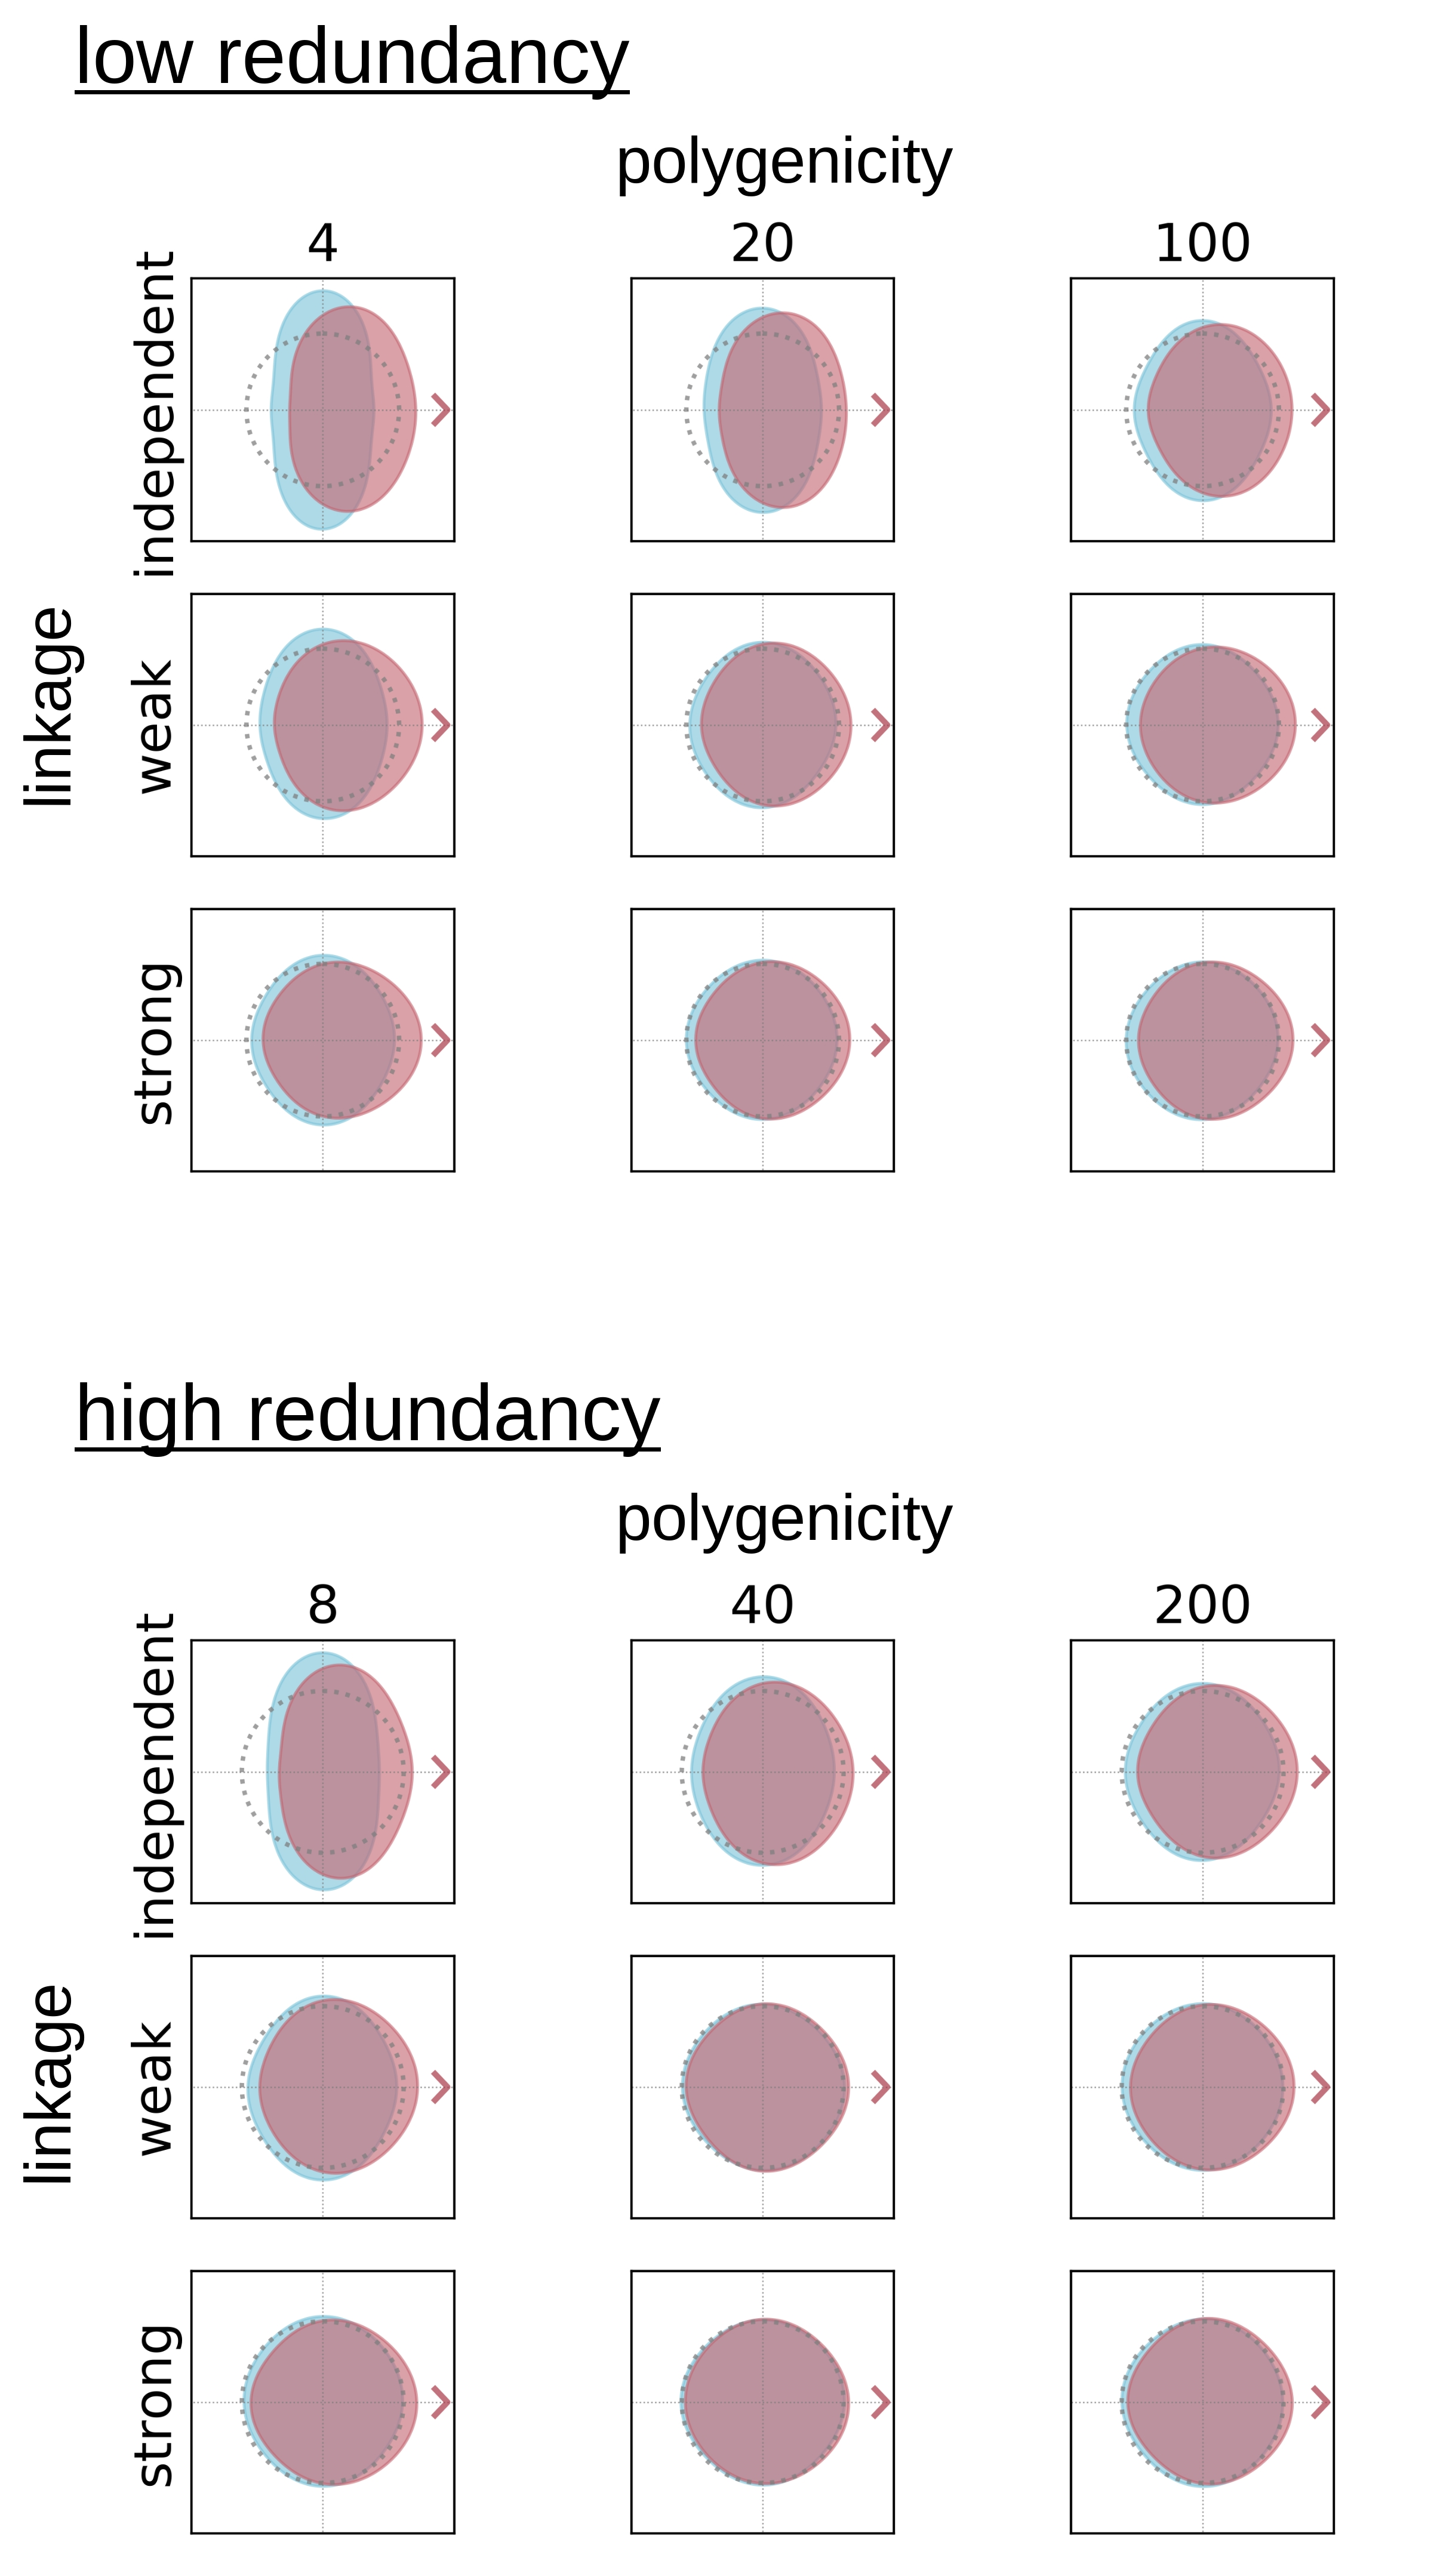
\includegraphics[width=.8\linewidth]{pub/figs/FIG_2_gene_flow.jpg}
    \caption{Comparison, across all 18 scenarios, of the distributions of gene-flow directions during the climate change period. Scenarios are organized into top and bottom sections for low and high redundancy, with rows in each section representing levels of linkage and columns representing polygenicity. Main scenarios (red) are compared against null scenarios (blue). Compass labels indicate directions of gene flow as it would be observed from a bird’s-eye view of the simulated landscape, with rightward (i.e., `up-gradient') gene flow moving in the same direction as the shifting environmental gradient, and with upward and downward (i.e., `on contour’) gene flow being perpendicular to the environmental gradients. Down-gradient gene flow is expected to be maladaptive under all scenarios, explaining why it is universally suppressed relative to the null results. There is a general trend toward increasing on-contour gene flow and decreasing up-gradient gene flow with decreasing strength of linkage and increasing number of loci per trait.
}
\label{fig:fig_2}
\end{figure}


\subsection{Linkage and polygenicity}
As expected, our null simulations showed essentially no changes
in mean fitness (Fig. \ref{fig:fig_2}) or population size(Fig. \ref{fig:fig_s2})
--- aside from small modeling artefacts that applied to both
null and climate-change scenarios --- and their phenotypic distributions were
stable through time (Fig. \ref{fig:fig_s3}).
The results of our climate change simulations exhibited the 
predicted decreases in population size and mean fitness
that are the expected results of maladaptation \cite{aitken_whitlock}.
They also revealed environment-tracking bivariate phenotypic shifts (Fig. \ref{fig:fig_4})
in line with the expected direction depicted in the lower half of Fig. \ref{fig:fig_1}
but with variable amounts of shortfall below the fitness-maximizing phenotypic shift.
Across scenarios, the demographic impacts of
climate change increased with increasing linkage
(change in fitness: $\beta_{l} = -0.00183\pm0.00010, P<2\times10^{-16}$;
change in population size: $\beta_{l} = -33.33\pm1.287, P<2\times10^{-16}$;
maladaptation (i.e., area of phenotypic-shift shortfall): $\beta_{l} = 0.0038\pm0.0004, P<2\times10^{-16}$).
Demographic impacts also showed a signal of overall increase with increasing polygenicity
(change in fitness: $\beta_{p} = -0.00217\pm0.00010, P<2\times10^{-16}$;
change in population size: $\beta_{p} = -15.07\pm1.287, P<2\times10^{-16}$;
maladaptation: $\beta_{p} = 0.0097\pm0.0004, P<2\times10^{-16}$);),
although the cross-scenario trend was non-monotonic and complex: impacts were smallest at moderate polygenicity;
more pronounced at low polygenicity and at high polgenicity when redundancy was high;
and extreme at high polygeniciy and low redundancy (Fig. \ref{fig:fig_3}, Fig. \ref{fig:fig_s2}).
Indeed, demographic decline was so strong at low redundancy and high polygenicity
that adaptive capacity was effectively outstripped: demographic decline persisted throughout
the climate change period, with little indication of evolutionary rescue
(i.e., stabilization and rebound) occurring until the post-change period (see Fig. \ref{fig:fig_3}, Fig. \ref{fig:fig_s2}).
The collapse of adaptive capacity in these scenarios
is also visible in the large red areas of phenotypic-shift shortfall in Fig. \ref{fig:fig_4}.
The low-redundancy, high-polygenicity, strong-linkage scenario had such low adaptive capacity
that mean fitness declined by 5.2\% on average (from 0.934 to 0.885),
mean population size declined by 17.1\% on average (from 6326 to 5246 individuals),
and the simulated population ceased to occupy the rightmost, fastest-changing portion of the landscape.
This is visible as the disappearance of population density in the portion
of the post-climate change phenotypic space corresponding to that region of the landscape in Fig. \ref{fig:fig_4},
but is more clearly visible in the before-after population density maps \ref{fig:fig_s4}.

\begin{figure*}[\sidecaptionrelwidth][t]
\centering
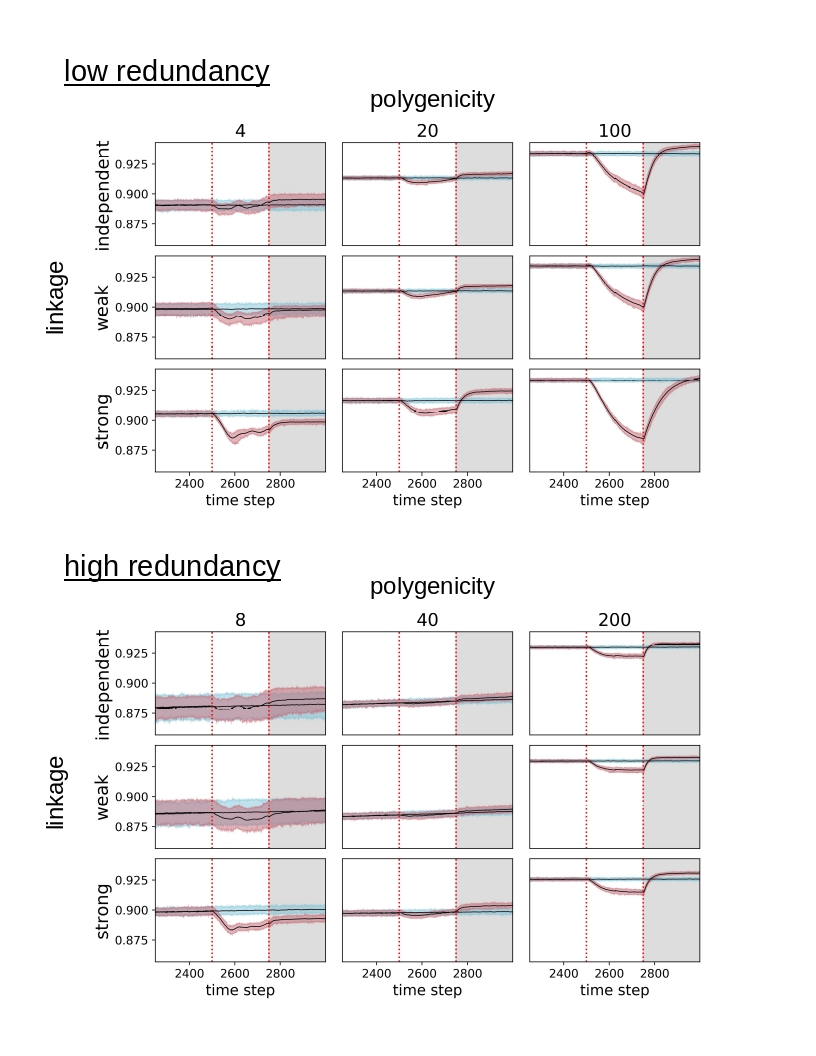
\includegraphics[width=17.8cm]{pub/figs/FIG_3_fit_over_time.jpg}
\caption{Left: Mean fitness dynamics for all scenarios during the 250 time steps before the climate change period and the 250 time steps during it (with the two periods divided by a red, dashed vertical line marking the onset of the climate change period). Scenarios are organized as in Fig. \ref{fig:fig_2}: top and bottom sections for low and high redundancy, with rows in each section representing levels of linkage and columns representing polygenicity. Right: Comparison of climate change-driven changes in mean fitness across scenarios. Null scenarios are plotted on the left in blue, and main scenarios are plotted on the right, in red. Within each plot, scenarios are divided by the number of loci per trait (x-axis) and by the strength of linkage (shade, with darker hues representing stronger linkage). Asterisks above each box indicate level of significance (*=0.1, **=0.05, ***=0.005).}
\label{fig:fig_3}
\end{figure*}

\begin{figure*}
\centering
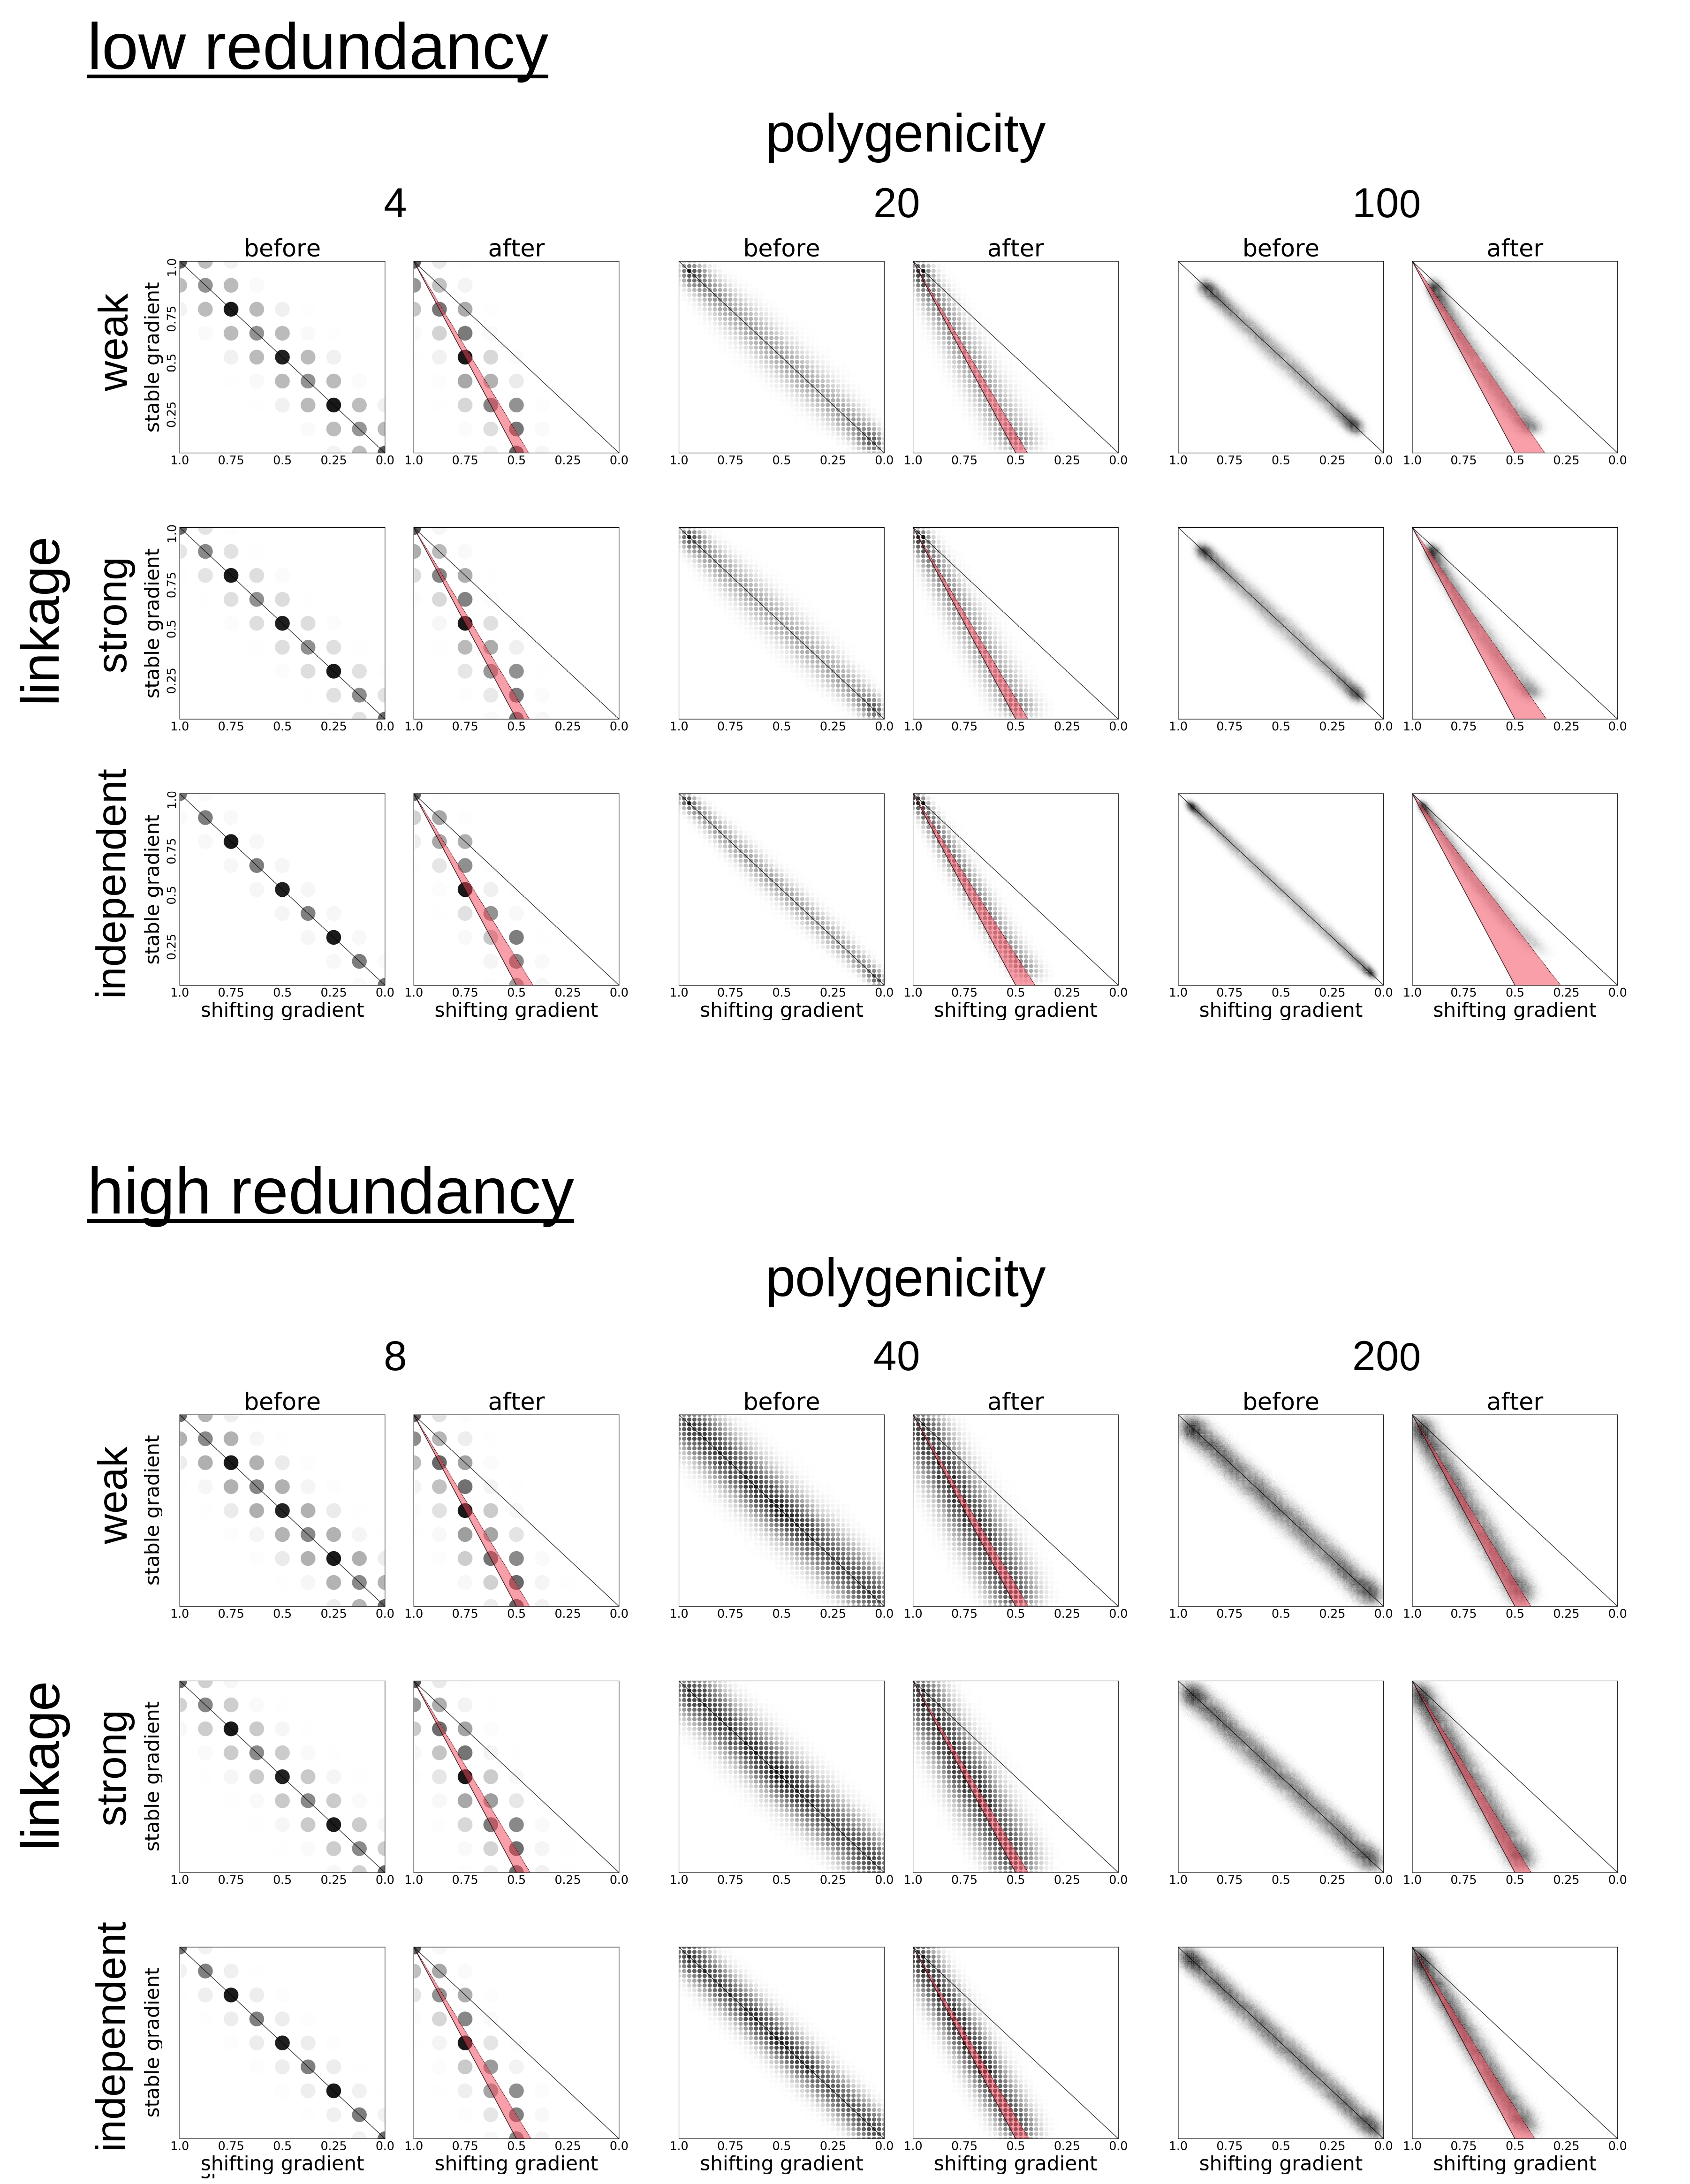
\includegraphics[width=15.8cm]{pub/figs/FIG_4_phenotypic_shift.jpg}
\caption{Comparison, across all 18 redundancy scenarios, of the observed versus expected phenotypic shift during the climate change period. Scenarios are organized as in Fig. \ref{fig:fig_2}: top and bottom sections representing low and high redundancy, with rows in each section representing levels of linkage and columns (in before-after pairs) representing polygenicity. For each scenario, the left ('before') scatterplot shows the distribution of individuals’ bivariate phenotypes before climate change begins, whereas the right ('after') scatterplot shows how the distribution has shifted by the end of the climate change period. The trait adapted to the shifting environmental gradient is distributed along the x axis, and the trait adapted to the stable gradient is distributed along the y axis. Scatterplots depict multi-model ensemble results for each scenario. The size and opacity of each point represents the number of individuals exhibiting that bivariate phenotype. (Note that the gridded arrangement of the points in each scatterplot is a function of the number of loci per trait which, because locus effect sizes are fixed, directly determines the set of attainable, evenly-spaced, discrete phenotypic values. Because fewer loci per trait yields fewer possible phenotypes, individuals are grouped into fewer, larger phenotypic bins in the 4- and 20-locus scenarios.) Solid black lines delineate the shift in the phenotypic distributions’ central tendencies that is expected to take place during the cimate change period, dotted black lines depict the observed (OLS-fitted) phenotypic distributions’ central tendencies at the ‘during’ and ‘after’ time steps, and translucent red wedges depict the differences between the expected and observed distributions (i.e., ‘phenotypic shortfall’, the response variable in our statistical tests).
}
\label{fig:fig_4}
\end{figure*}
 

\subsection{Genotypic redundancy}
Our high-redundancy scenarios showed
consistently smaller demographic impacts of climate change and higher adaptive capacity
than their low-redundancy counterparts 
(change in fitness: $\beta_{r} = 0.00402\pm0.00016, P<2\times10^{-16}$;
change in population size: $\beta_{r} = 39.06\pm2.101, P<2\times10^{-16}$;
maladaptation: $\beta_{r} = -0.0098\pm0.0006, P<2\times10^{-16}$), supporting our hypothesis that
genotypic redundancy can facilitate adaptation to shifting environmental gradients (Fig. \ref{fig:fig_2}, Fig. \ref{fig:fig_s2}).
This effect was most pronounced in the high-polygenicity scenarios,
which exhibited much milder demographic decline under high redundancy,
despite still showing no evidence of demographic rebound until after climate change (Fig. \ref{fig:fig_3}).
Indeed, increased redundancy put the demographic
impacts of these scenarios on par with those
of the low-polygenicity scenarios (e.g., compare
low- and high-redundancy boxplots in Fig. \ref{fig:fig_3} and Fig. \ref{fig:fig_s2}).


\section*{Discussion}

Current theoretical understanding of evolutionary responses to climate change
largely derives from a simplified mechanistic model in which
adaptation is universally facilitated by up-gradient gene flow.
This model is not only the conceptual basis for research
but also the inspiration for some climate-smart
approaches to biodiversity management
(e.g., assisted gene flow; \cite{aitken_whitlock}).
However, by employing this model as the basis
for theoretical and mechanistic research
we risk overlooking the nuanced but important dynamics that
can result when complex genomic architectures
are involved in local adaptation
to multivariate environmental change.
Starting from this more realistic framework,
our simulations confirm that up-gradient gene flow does, indeed,
play a generalized role in mitigating
the impacts of climate change on populations,
but they also reveal a major caveat:
polygenicity and, to a lesser extent, linkage
can limit the extent to which
gene flow contributes to adaptation.
Given the plausibility of the range of genomic architectures we simulate
\cite{barghi_polygenic,boyle,rockman,savolainen,sella,bomblies},
these results raise the compelling
possibility that up-gradient gene flow, while unlikely
to be maladaptive, could nonetheless prove
ineffectual for supporting adaptation in many systems,
especially those where climate-adapted traits
have more dispersed architectures
(i.e., architectures composed of many genes of small effect; \cite{yeaman_review}),
providing a higher capacity for \textit{in situ} adaptation to rapid change.
This poses an important question for subsequent research:
How often are climate-adapted trait architectures dispersed,
versus being more concentrated (i.e., composed of
few loci of large effect)?

The genomic architecture of climate-adapted traits
also has the potential to influence the population dynamics
that occur during evolutionary responses to climate change.
Our results show that neglecting this fact
can lead to overlooking important contingencies,
whereas accounting for them can extend current theory and provide valuable insight.
First, our results suggest that strong linkage between non-neutral loci,
especially under high polygenicity, can increase maladaptation and demographic decline
during climate change. 
In the most extreme case, high polygenicity and low redundancy
combine to drive dramatic and persistent declines
and even local extinction when linkage is strong.
This was unexpected in light of previous work reporting
that dispersed architectures produce stable,
resilient phenotypic clines despite transient genotypic composition \cite{yeaman_amnat,yeaman_review},
and thus that species with such architectures
could exhibit rapid local adaptation \cite{aitken_yeaman}. 
We still expected evolutionary responses to climate change
to be slower in these scenarios,
because natural selection is less effective on smaller-effect alleles
and because high linkage leads to longer expected wait times for the generation
of novel, adaptive recombinants, but we did not expect
to see such a pronounced lack of adaptive capacity.
The fact that high genotypic redundancy reduces demographic decline,
not just in these but across all scenarios, contributes to the building recognition of the importance of redundancy
as a driver of population-genetic outcomes in polygenic systems
\cite{laruson,yeaman_review},
and also presents a possible mechanism to be explored
in real-world populations living at species' colder range edges.
Much like the local populations in the rightmost region of our low-redundancy scenarios,
these populations could already be at the edge of the phenotypic space defined by
standing genetic variation, such that local selection would be directional,
segregating redundancy (\textit{a la} \cite{laruson}) correspondingly low,
adaptive capacity lacking, and extinction vulnerability substantial.
However, species whose cold range edges are more determined by geographic barriers
or biotic interactions than by bioclimate \cite{thomas}
could feature populations more similar to our high-redundancy scenarios:
selection would be balancing rather than directional,
segregating redundancy substantial, and thus adaptive capacity more robust.

Our findings also help advance the theoretical understanding
of local adaptation with recombination.
Recombination is generally regarded as disadvantageous
in situations of clinal adaptation
with gene flow, because it disrupts the association between adaptive loci 
underlying a single trait,
but unstable environments are considered a major exception \cite{tigano}.
Our results suggest that recombination can also
be advantageous under the monotonic environmental
change that is characteristic of climate change,
particularly when simultaneous adaptation is occurring
for multiple traits adapted to decoupling gradients.
This likely occurs because recombination
allows for more effective \textit{in situ} adaptation
by shifting allelic covariance --- despite the fact that
it still disrupts the associations between loci
that would otherwise allow for the development of
larger-effect gene clusters.
 
Second, the minimal demographic decline
in our moderate-polygenicity models
contrasts with previous work finding that adaptation
to a gradient is more effective under either
concentrated or dispersed genomic architectures \cite{yeaman_whitlock}.
This disagreement may be attributable to the
difference in timeframes between adaptation to a univariate environmental gradient
and adaptation to a decoupling, multivariate gradient.
Adaptation to a single, static gradient can proceed gradually,
so may either favor large-effect alleles or allele-clusters in the long haul
\cite{yeaman_amnat,yeaman_review},
once they have arisen by mutation, recombination, gene flow, or a combination thereof,
or dispersed architectures 
\cite{burger,kondrashov,yeaman_review,yeaman_whitlock}
in temporally fluctuating environments.
However, the sudden onset of persistent environmental change 
in a population that is already locally adapted triggers a 'race against time,' 
and it may be that the genetic architectures with
optimal adaptive capacity are 'middle ground' architectures that comprise
freely recombining loci with small-enough effect sizes to avoid large
sudden declines in fitness from migration load
but with large enough effect sizes to avoid the long wait times necessary
for recombination to cluster many adaptive loci into larger-effect haplotypes.
If this is true it would suggest an inherent tension between the architectures that
might be expected to evolve in locally adapted populations prior to climate change
and those most likely to facilitate adaptation to change --- although
the precise intragenomic positions of the loci involved,
left simplistically symmetric in our simulations, may be influential in real-world systems.
 
A major challenge in simulation-based research is the complexity of the high-dimensional 
parameter space that could be explored.
Informative studies can be constructed by focusing on a small set of
key parameters while holding others at reasonable values, as we have done here.
This nonetheless leaves unexplored a number of secondary parameters
that can have non-negligible influence over the complex ecological phenomena of interest.
In the case of evolutionary responses to climate change,
a number of these provide areas for future research, including:
population size, a key determinant of the relative strengths of drift
and natural selection \cite{murray} and of the wait time to emergence of
recombinant haploytpes \cite{christiansen}, among other important dynamics;
movement behavior, a key factor embedded in the rudimentary
migration-selection dynamics that lie at the heart of models like ours
\cite{wright,haldane,barton};
allelic effect size distributions \cite{orr},
which are omitted here in favor of a single fixed effect size but would
help clarify evolutionary tendencies when loci of varying effect sizes
are simultaneously subject to selection;
and the structure of the environment,
including the geometries, slopes, and orientations of gradients
(e.g., \cite{benes}) and their rates of change.
A number of other more complex evolutionary aspects could also be explored 
through a similar modeling framework, including 
pleiotropy \cite{thompson} and epistasis,
hybridization CITE, and life history variation.
Finally, important and conservation-relevant insight could emerge from the 
integration of other dimensions of climate change ecology, including range shifts 
\cite{weiss-lehman}, plasticity \cite{chevin},
and range-wide variation in population density \cite{aitken_whitlock}.

Adaptation is one of the main mechanisms by which species
have a chance of weathering climate change.
Given the decoupling of environmental gradients that
climate change will frequently cause,
adaptive responses will often be multivariate.
Within this context, the potential influence of adaptive genomic architecture
on evolutionary outcomes has typically been neglected in conceptual and mechanistic models.
Our results show that this neglect leads
us to overlook important variability in the nature
and success of adaptive responses,
including strong influence of genomic architecture
on both the effectiveness
of up-gradient gene flow and the magnitude and persistence
of maladaptation and concomitant demographic decline.
Further research in this arena, both simulated and empirical,
can help refine our understanding of adaptation to climate change,
both advancing evolutionary theory
and facilitating the development of better-informed management strategies.


\matmethods{

\subsection*{Simulation}

We performed all of the simulations for this study using \texttt{geonomics} \cite{terasaki_hart},
a Python \cite{rossum} package for
creating forward-time, agent-based, continuous-space landscape genomic simulations 
using arbitrarily complex life histories, environments, and environmental change 
scenarios. All of our simulated scenarios feature
a species with two traits, each of which experiences 
selection on the basis of a different environmental variable.
Both environmental variables are modeled as linear, horizontal gradients
that initially span environmental values from 1 to 0, left to right.
The fitness of individuals is a function of the difference between their local
environmental values and their phenotypes, which are determined by the
additive effects of multiple loci (i.e., without pleiotropy or epistasis) ---
a reasonable approximation of many traits of interest in real populations \cite{sella}.

Each simulation starts with a neutral burn-in period, ended by \texttt{geonomics}' tests
of temporal and spatial population stability, then runs for 2500 time steps
non-neutral evolution, generating a pattern of local adaptation to the initial environment.
After that, one of the environmental layers undergoes a change 
event in which the gradient’s values change stepwise over a period of 250 time steps,
resulting in a final gradient that spans values from 1 to 0.5, left to right.
This creates a scenario in 
which the two environmental variables become decoupled, leading 
to the emergence of novel environments (i.e. sites occupying new vectors in 
two-dimensional environmental space).
The purpose of this is to emulate a common 
phenomenon under climate change: the decoupling of multivariate environmental gradients,
leading to the emergence of novel climates
\cite{williams_novel_climates,williams_projected_novel_disappearing,fitzpatrick_climate_novelty_forecasts}.
Importantly, this landscape arrangement generates heterogeneous rates of climate change,
with the rate ranging from 0 at the leftmost edge to $\frac{0.5}{250 time steps}$ at the rightmost edge.
This complicates interpretation of our results,
but less so than in an alternative scenario
with spatially homogeneous rates of change,
which would generate an artefact of range expansion
whose genomic signal would be superimposed on that of
climate change adaptation.
This latter approach is also of interest,
and may be explored in future work,
but the approach we chose here allows us
to best isolate the evolutionary dynamics
resulting from the components of genetic architecture
that define our scenarios and hypotheses.

Next, we wrote a custom Python script that reads the template \texttt{geonomics}
parameters file, edits any parameters that vary 
across our scenarios, instantiates a model, runs a fixed number of iterations 
of that model, and outputs simulated genetic and other data. 
Our parameters of interest are the number of loci underlying
each trait (parameter \texttt{n\_loci}),
the linkage between neighboring loci
(i.e., the homogeneous recombination rate; parameter \texttt{recomb}),
and the amount of genotypic redundancy (parameter \texttt{redund}).
The values we assigned to these parameters are provided in Table \ref{tab:tab_1}.
Of note, in low-redundancy scenarios the \texttt{n\_loci} values we specify
produce many-to-one genotype-phenotype mappings at intermediate phenotypes
that decline to one-to-one mappings at extreme phenotypes,
whereas in high-redundancy scenarios the doubled \texttt{n\_loci} values
produce many-to-one mappings across all phenotypes between 0 and 1, inclusive
--- i.e., all phenotypes matching environmental values
that occur somewhere on the landscape.
The full factorial combinations of the chosen values of those parameters generate the set
of simulation scenarios depicted in the tabular arrangments of figures
Fig. \ref{fig:fig_2}, Fig. \ref{fig:fig_3}, Fig. \ref{fig:fig_4}, Fig. \ref{fig:fig_s2}, Fig. \ref{fig:fig_s3}, and Fig. \ref{fig:fig_s4}.
We used that script to run a set of batch jobs on the 
savio3 partition of UC Berkeley’s Savio system (each node has 96 GB RAM and 32, 
2.1-GHz Skylake processors). For each scenario, we ran a total of 100 iterations of 
the scenario of interest, featuring a 250-time-step climate change period (henceforth, 
the ‘main’ scenarios), and 100 iterations of a paired null scenario without natural 
selection (henceforth, the ‘null’ scenarios). 
Given that \texttt{geonomics} is a complex simulation framework, it features numerous other 
parameters, which we set at reasonable default values.
For the complete set of parameters and the values 
assigned to them across all models
(as well as green-highlighted notes denoting runtime and genomic-architecture
parameter overridden by the main simulation scripts), see Appendix 1.

Using a combination of internal \texttt{geonomics} functions and custom Python code, we 
designed a set of data outputs from each model run, to visualize our
results and test our series of hypotheses.
We saved tables of individuals’ locations and phenotypes at both
the beginning and the end of the climate change period. We also saved time 
series of population size, mean fitness, and mean phenotype of the trait adapted to 
the shifting gradient. We gathered this data at every time step, from 250 time steps 
before the onset of climate change, through the 250 time steps of the event, and 
continuing until 250 time steps after climate change completed.
The final 250 time steps after climate change are unrealistic, but are useful
for elucidating the nature of the changes that persisted to the end of the climate change period;
we refer to this period as the 'post-change period'.

We also saved subsampled data on the vector directions
of gene flow occurring during climate change, by keeping all final individuals'
data pertaining to two randomly chosen loci that had positive
effects on the trait adapted to the shifting environmental gradient.
We restricted our sample in this way both to focus on loci expected to facilitate 
adaptation to increasing environmental values and thus to shift up-gradient, and to 
provide equal sample sizes across scenarios in downstream analysis (which was 
constrained to the number of positive-effect loci present in
the low-polygenicity, low-redundancy scearnios). 
Data were collected using an internal \texttt{geonomics} function
that extracts data from the spatial pedigrees stored in the
simulation's \texttt{tskit} \cite{kelleher} data structures.
We also calculated a single high-level summary metric per model
that provided us a comparator for the relative amounts of
up-gradient gene flow that occurred across our scenarios,
for use in hypothesis testing.
We refer to the metric simply as 'up-gradient gene flow',
and we calculate it as:

$GF_{up}\ = \frac{\sum\limits_{i}^{n}\cos\theta}{n},\ \cos\theta\geq0$,

where angles are expressed counterclockwise from the right.
The $\cos\theta\geq0$ condition allows us to ignore leftward gene flow,
which we expected to be low irrespective of scenario for the positive-effect loci
for which we collected data,
given that it would oppose the environmental shift so would be generally maladaptive.


\subsection*{Analysis}

We analyzed all 18 scenarios' and all 100 iterations' data
using visual summaries and companion statistical tests.
All analysis and visualization was produced using custom scripts written in 
Python and R \cite{r_core_team}.

To test our first hypothesis about gene flow,
we first produced a visualization of the directional 
distributions of gene flow in all 18 scenarios, comparing between main
and null scenarios (Fig. \ref{fig:fig_2}).
To create this visualization, we gathered directional data
from each simulation for a random 
sample of the gene flow that occurred during the climate change event, using 
\texttt{geonomics}' integration with \texttt{tskit} \cite{kelleher}, which allows for temporal 
subsetting and output of the information contained the full spatial pedigree of a 
simulated population. We then fitted a mixture of 4 von Mises distributions to that data
using the R package \texttt{movMF} \cite{hornik},
yielding 12 parameter estimates defining each simulation's fitted mixture distribution. For each of 
the 18 scenarios, we then plotted the probability density function 
described by the means of all length-12 vectors of fitted parameters. We did this 
separately for null scenarios and for main scenarios, then overlaid the main scenario (in red)
on top of the nulls (in blue), providing a summary depiction of the nature of gene flow within each 
main scenario as compared to its null expectation.

Finally, we ran a simple linear regression
of the main-null difference in up-gradient gene flow density
as a function of the components of genomic architecture
($GF_{up,main}-GF_{up,null} \sim \alpha + \beta_{p}polgenicity + \beta_{l}linkage + \beta_{r}redundancy + \epsilon$),
which we used to interpret our results and test the components of our first hypothesis.
We model the genomic architecture components
as numeric integer variables
representing the factorial or exponential increases
used to set their parameter values in simulations:
polygenicity: low = 0, moderate = 1; high = 2 ($polygenicity_{variable}=\log_{5}(\frac{polygenicity_{simulated}}{4\times\ redundancy_{variable}})$;
linkage: low = 0, moderate = 1, high = 2 ($linkage_{variable}=-\log_{10}(\frac{linkage_{simulated}}{0.5})$);
redundancy: low = 0, high = 1.
We use this model, compared against
the patterns revealed by Fig. \ref{fig:fig_2},
to test both components of our first hypothesis,
expecting all scenarios' fitted values
for the main-null difference in up-gradient gene flow
to have 95\% confidence intervals $>0$ for the main-null difference in up-gradient gene flow (component 1),
and expecting the coefficients on the linkage and polygenicity
terms of the model to be significantly positive and
negative, respectively (component 2).

To visually assess our second and third hypotheses, we created a series of
plots comparing climate change-driven demographic shifts
and maladptation across all 18 scenarios and between null and main moels.
First, we plotted the 
null and main trajectories of two demographic
metrics --- mean fitness and population size --- in 
each of our 18 scenarios. For each scenario and metric, and 
for both main and null models, we created ensemble datasets by combining all 100 
iterations’ output time series of the metric,
then derived summary time series by calculating each time step's
100-iteration mean and 5th and 95th percentiles.
We plotted the resulting summary time series in Fig. \ref{fig:fig_3} (mean fitness)
and Fig. \ref{fig:fig_s2} (population size), with null results again shown in blue
and main results in red.
We plotted the metrics starting from 250 time steps before the climate change event
and running until 250 time steps after its completion, allowing us
to evaluate the onset, course, and aftermath of the demographic responses.
Additionally, we summarized all scenarios in a pair of box plots
(one plot for low genotypic redundancy, one for high),
with plots arranged by polygenicity along the x-axis,
colored blue or red to denote null or main results,
and shaded darker for increasing levels of linkage.

Next, to better understand changes in population size and distribution,
we mapped before-after comparisons of population density across all 18
main scenarios (Fig. \ref{fig:fig_s4}).
Each population density map is calculated as
the array of mean population densities at all cells on the landscape,
averaged across all 100 main simulations of the map's corresponding scenario.
Population densities are depicted as increasing from black to white, with
values standardized across the entire plot grid.

Finally, to visualize maladaptation, we created an identically-structured
grid of plots comparing each scenario's
mean phenotypic distributions before and after climate change,
including scatter plots of the density of individuals occuring across
two-dimensional trait space and lines and wedges depicting the average maladaptation
observed across each scenario's 100 iterations (Fig. \ref{fig:fig_4}).
We refer to the wedge as 'persistent maladaptation',
and we calculate it as the difference between: a.) the area 
within two-dimensional trait space that the population’s phenotypic distribution 
would have needed to shift through during the climate change event, so as to remain 
optimally fit to its environment, and b.) the observed area of phenotypic shift within
a scenario's 100 simulations.
(We qualify this metric as 'persistent' to emphasize that it does
not reflect transient maladaptation that arises but then
resides during the period of climate change, but rather reflects
only maladaptation that remains at the end of the climate change period.)
To measure this area, we first determined the triangular area between 
the expected central tendency lines of the optimal bivariate phenotypic distributions
before and after the climate change event;
these are unambiguously determined by the model parameterization, because
they are the lines connecting all of the discrete 
points in environmental space that occur on the pre- and post-change landscapes.
Then, for each model run, we used ordinary least squares (OLS)
to fit a central tendency line to the 100-iteration ensemble phenotypic distribution
observed at the end of the climate change event
(arithmetically fixing the y-intercept at the (1,1) point in phenotypic 
space, the unchanging phenotypic optimum at the leftmost extent of the landscape).
The area of the wedge between the expected and observed post-change central tendency
lines provides our measure of a scenario's persistent maladaptation.
We plot before and after scatter plots of the ensemble datasets
of individuals' two-dimensional phenotypes
(binned to a grid of regular points for interpretability, with points
shaded to depict relative densities of individuals).
We then overplot onto those scatter plots the central tendency lines of
the expected (dotted lines) and observed (solid lines) phenotypic distributions,
as well as the wedges of persistent maladaptation.
In Fig. \ref{fig:fig_s3} we produce the same plot as Fig. \ref{fig:fig_4},
but using data from null simulations to demonstrate that all differences
in maladaptation observed between scenarios were attributable to climate change,
and with blue translucent wedges showing the expected area of phenotypic shift
under each null scenario's corresponding main simulation, for reference.

To summarize our results,
we ran identically structured simple linear regressions
for each of our three response variables measuring
population-level changes during the climate change event
change in mean fitness, change in population size,
and persistent maladaptation --- with polygenicity,
linkage, redundancy, and nullness serving as explanatory variables:
$[\Delta N_{t}\ |\ \Delta fit\ |\ maladaptation] \sim \alpha + \beta_{p}polgenicity + \beta_{l}linkage + \beta_{r}redundancy + \beta_{n}nullness + \epsilon$.
We model nullness as a binary categorical variable (null=0, main=1)
and again model the genomic architecture components
as numeric integer variables, as described above.
We use these models, in combination with the
cross-scenario trends visible in
Fig. \ref{fig:fig_3}, Fig. \ref{fig:fig_s2}, and Fig. \ref{fig:fig_4},
to test the components of our second hypothesis
(polygenicity and linkage) and third (redundancy).
Specifically, our second hypothesis predicts that
the coefficients of the linkage and genicity terms are significantly
non-zero and negative (for the fitness-change
and population size-change models) or positive (for the maladaptation
model) with increasing linkage and genicity,
while our third hypothesis predicts significantly non-zero
redundancy coefficients with the opposite signs.

} % end matmethods




\showmatmethods{} % Display the Materials and Methods section

\acknow{We thank A. Bishop, T. Dawson,  J. Frederick, N. Graham, M. Kelly, M. McElroy, E. Westeen, G. Wogan, and M. Yuan for feedback and guidance on various iterations of the simulations presented herein. We thank Berkeley Research Computing for providing access to the Savio computing cluster. We thank D. Ehrenfeld, N. Fefferman, M. Fitzpatrick, and L. Plough for cultivating an interest in conservation genetics. Lastly, we thank M. Terasaki Hart, C. Nemec-Hart, G. Hart, J. Hart, and M. Tylka for supporting and encouraging a lifetime of curiosity about nature, and C. S. aTunde Adjuah, B. Evans, R. Pérez Joglar, Y. Y. Ma, and J. Redman for the pleasant solitude. This work was supported by a Berkeley Fellowship (to D.E.T.H.) and by National Science Foundation grant DEB1845682 (to I.J.W.).}

\showacknow{} % Display the acknowledgments section

% Bibliography
\bibliography{terasaki_hart_ch2}

%%%%%%%%%%%%%%%%%%%%%%%%%%%%%%%%%%%%%%%
% TEMPORARY PLACE FOR SUPPLEMENTAL FIGS

\pagebreak
\textbf{SUPPLEMENTAL FIGS:}


\begin{figure}
\centering
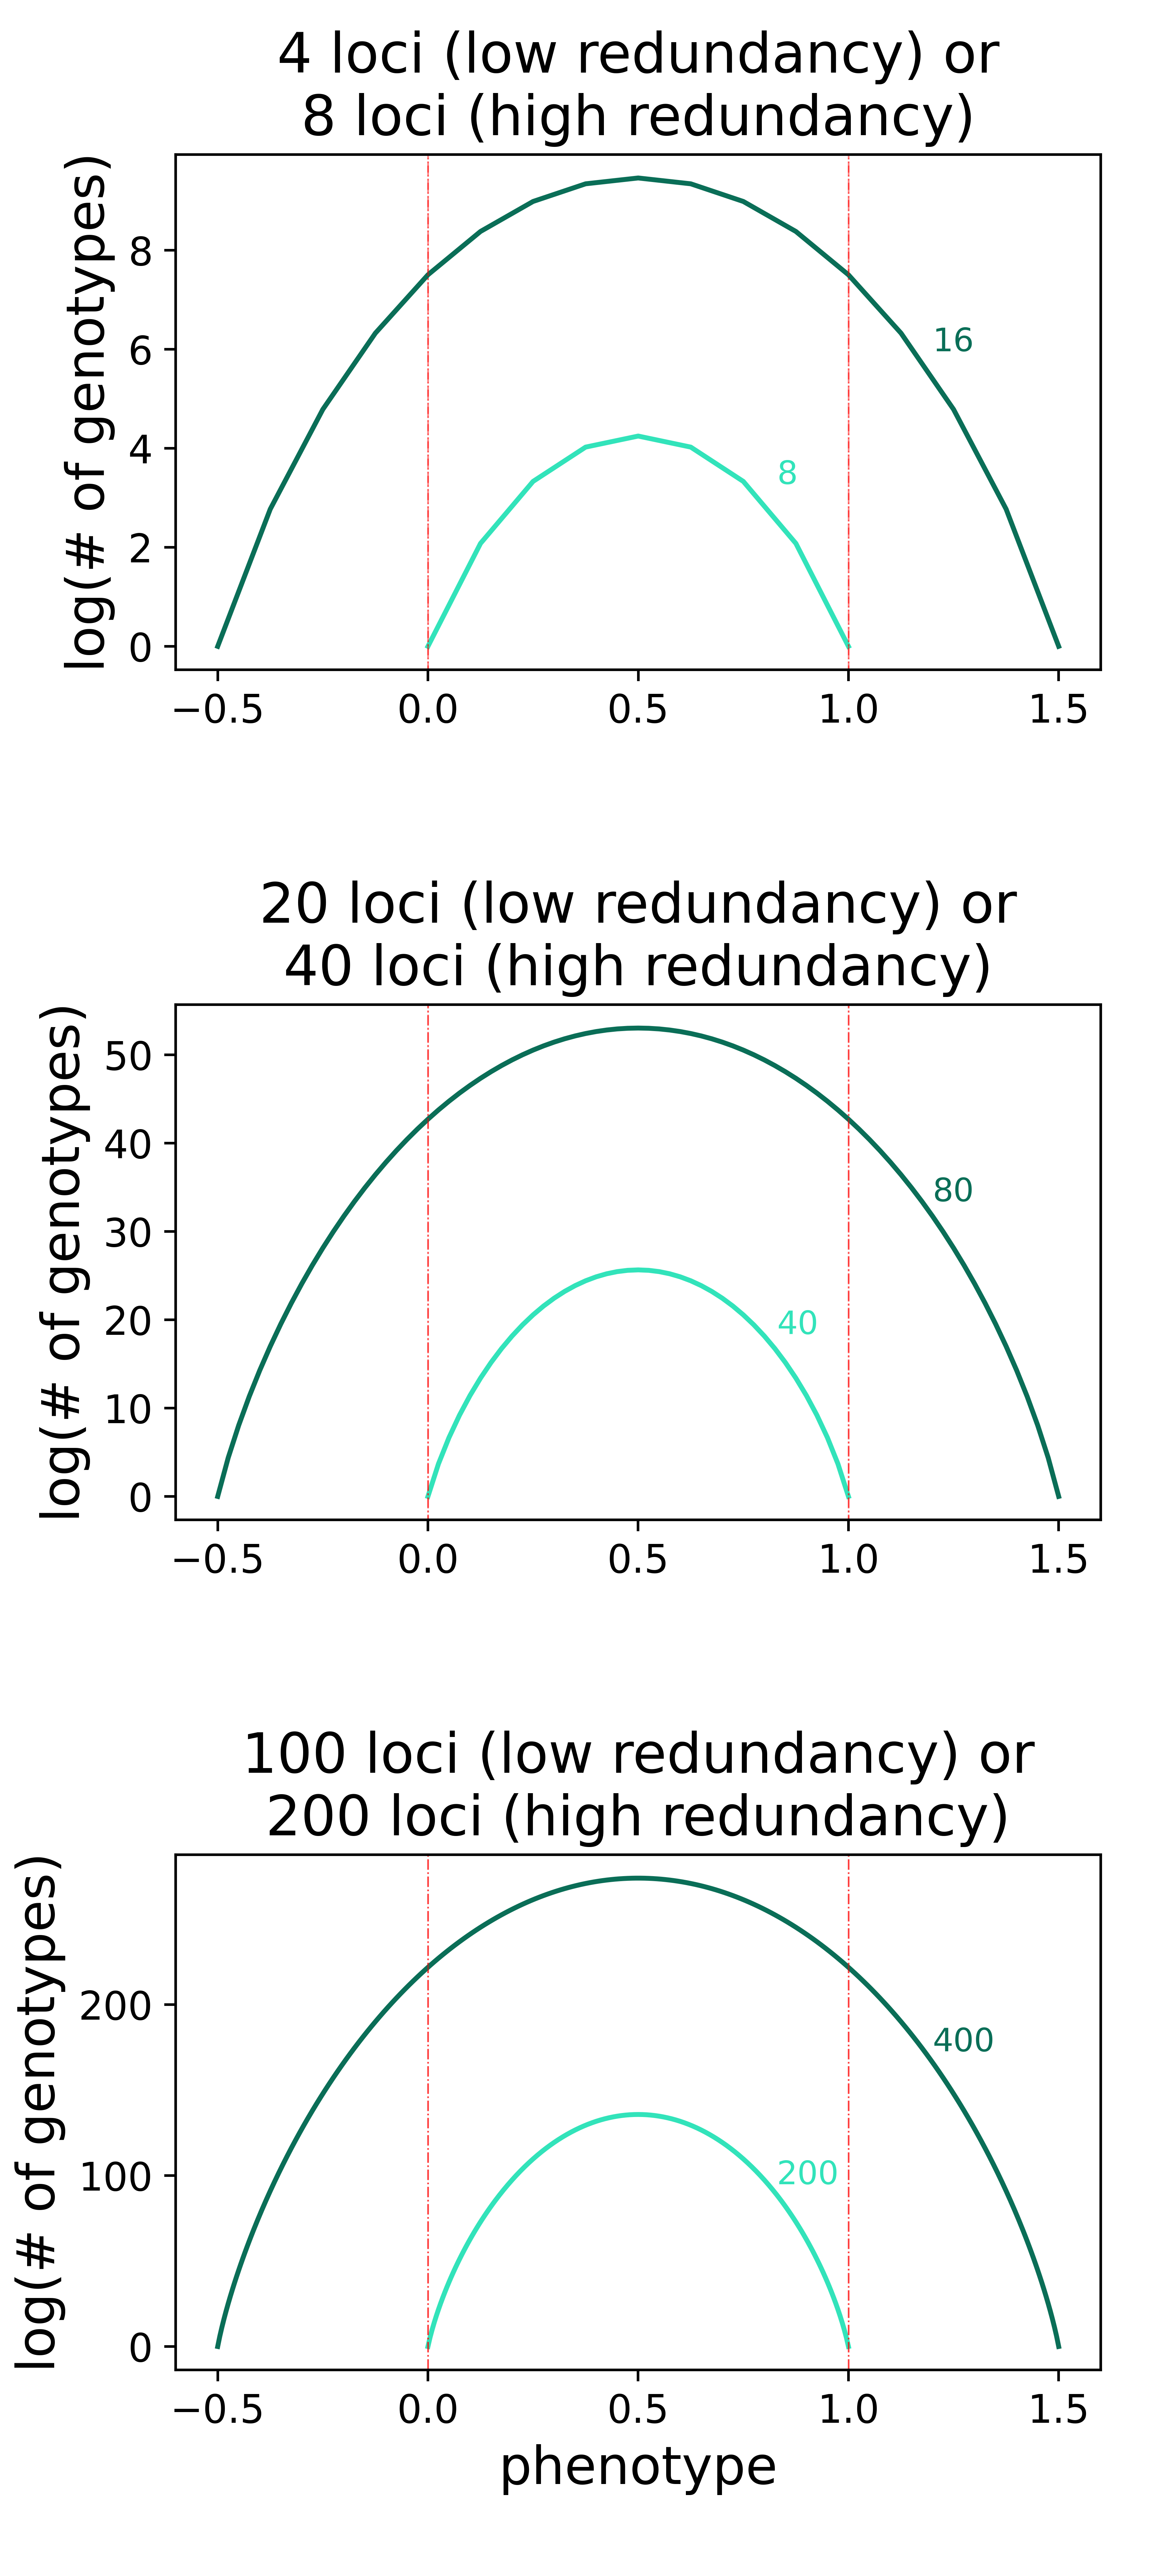
\includegraphics[width=.8\linewidth]{pub/figs/FIG_S1_redundancy.png}
\caption{Depiction of genotypic redundancy for all simulated polygenicity values. Phenotypic values are plotted along the x-axis, and the natural log of the number of genotypes that yield each phenotypic value is plotted along the y-axis. Polygenicities corresponding to low-redundancy scenarios are plotted and labeled in light teal, and those corresponding to high-redundancy scenarios in dark teal. The minimum and maximum environmental values on the landscape are represented by dotted vertical lines. The number of genotypes corresponding to each phenotype is calculated using a custom adaptation of Eqxn. ii, Box 1 in \cite{laruson}, implemented for a diploid species and fitted to the numerical conventions used by Geonomics.
}
\label{fig:fig_s1}
\end{figure}


\begin{figure*}[\sidecaptionrelwidth][t]
\centering
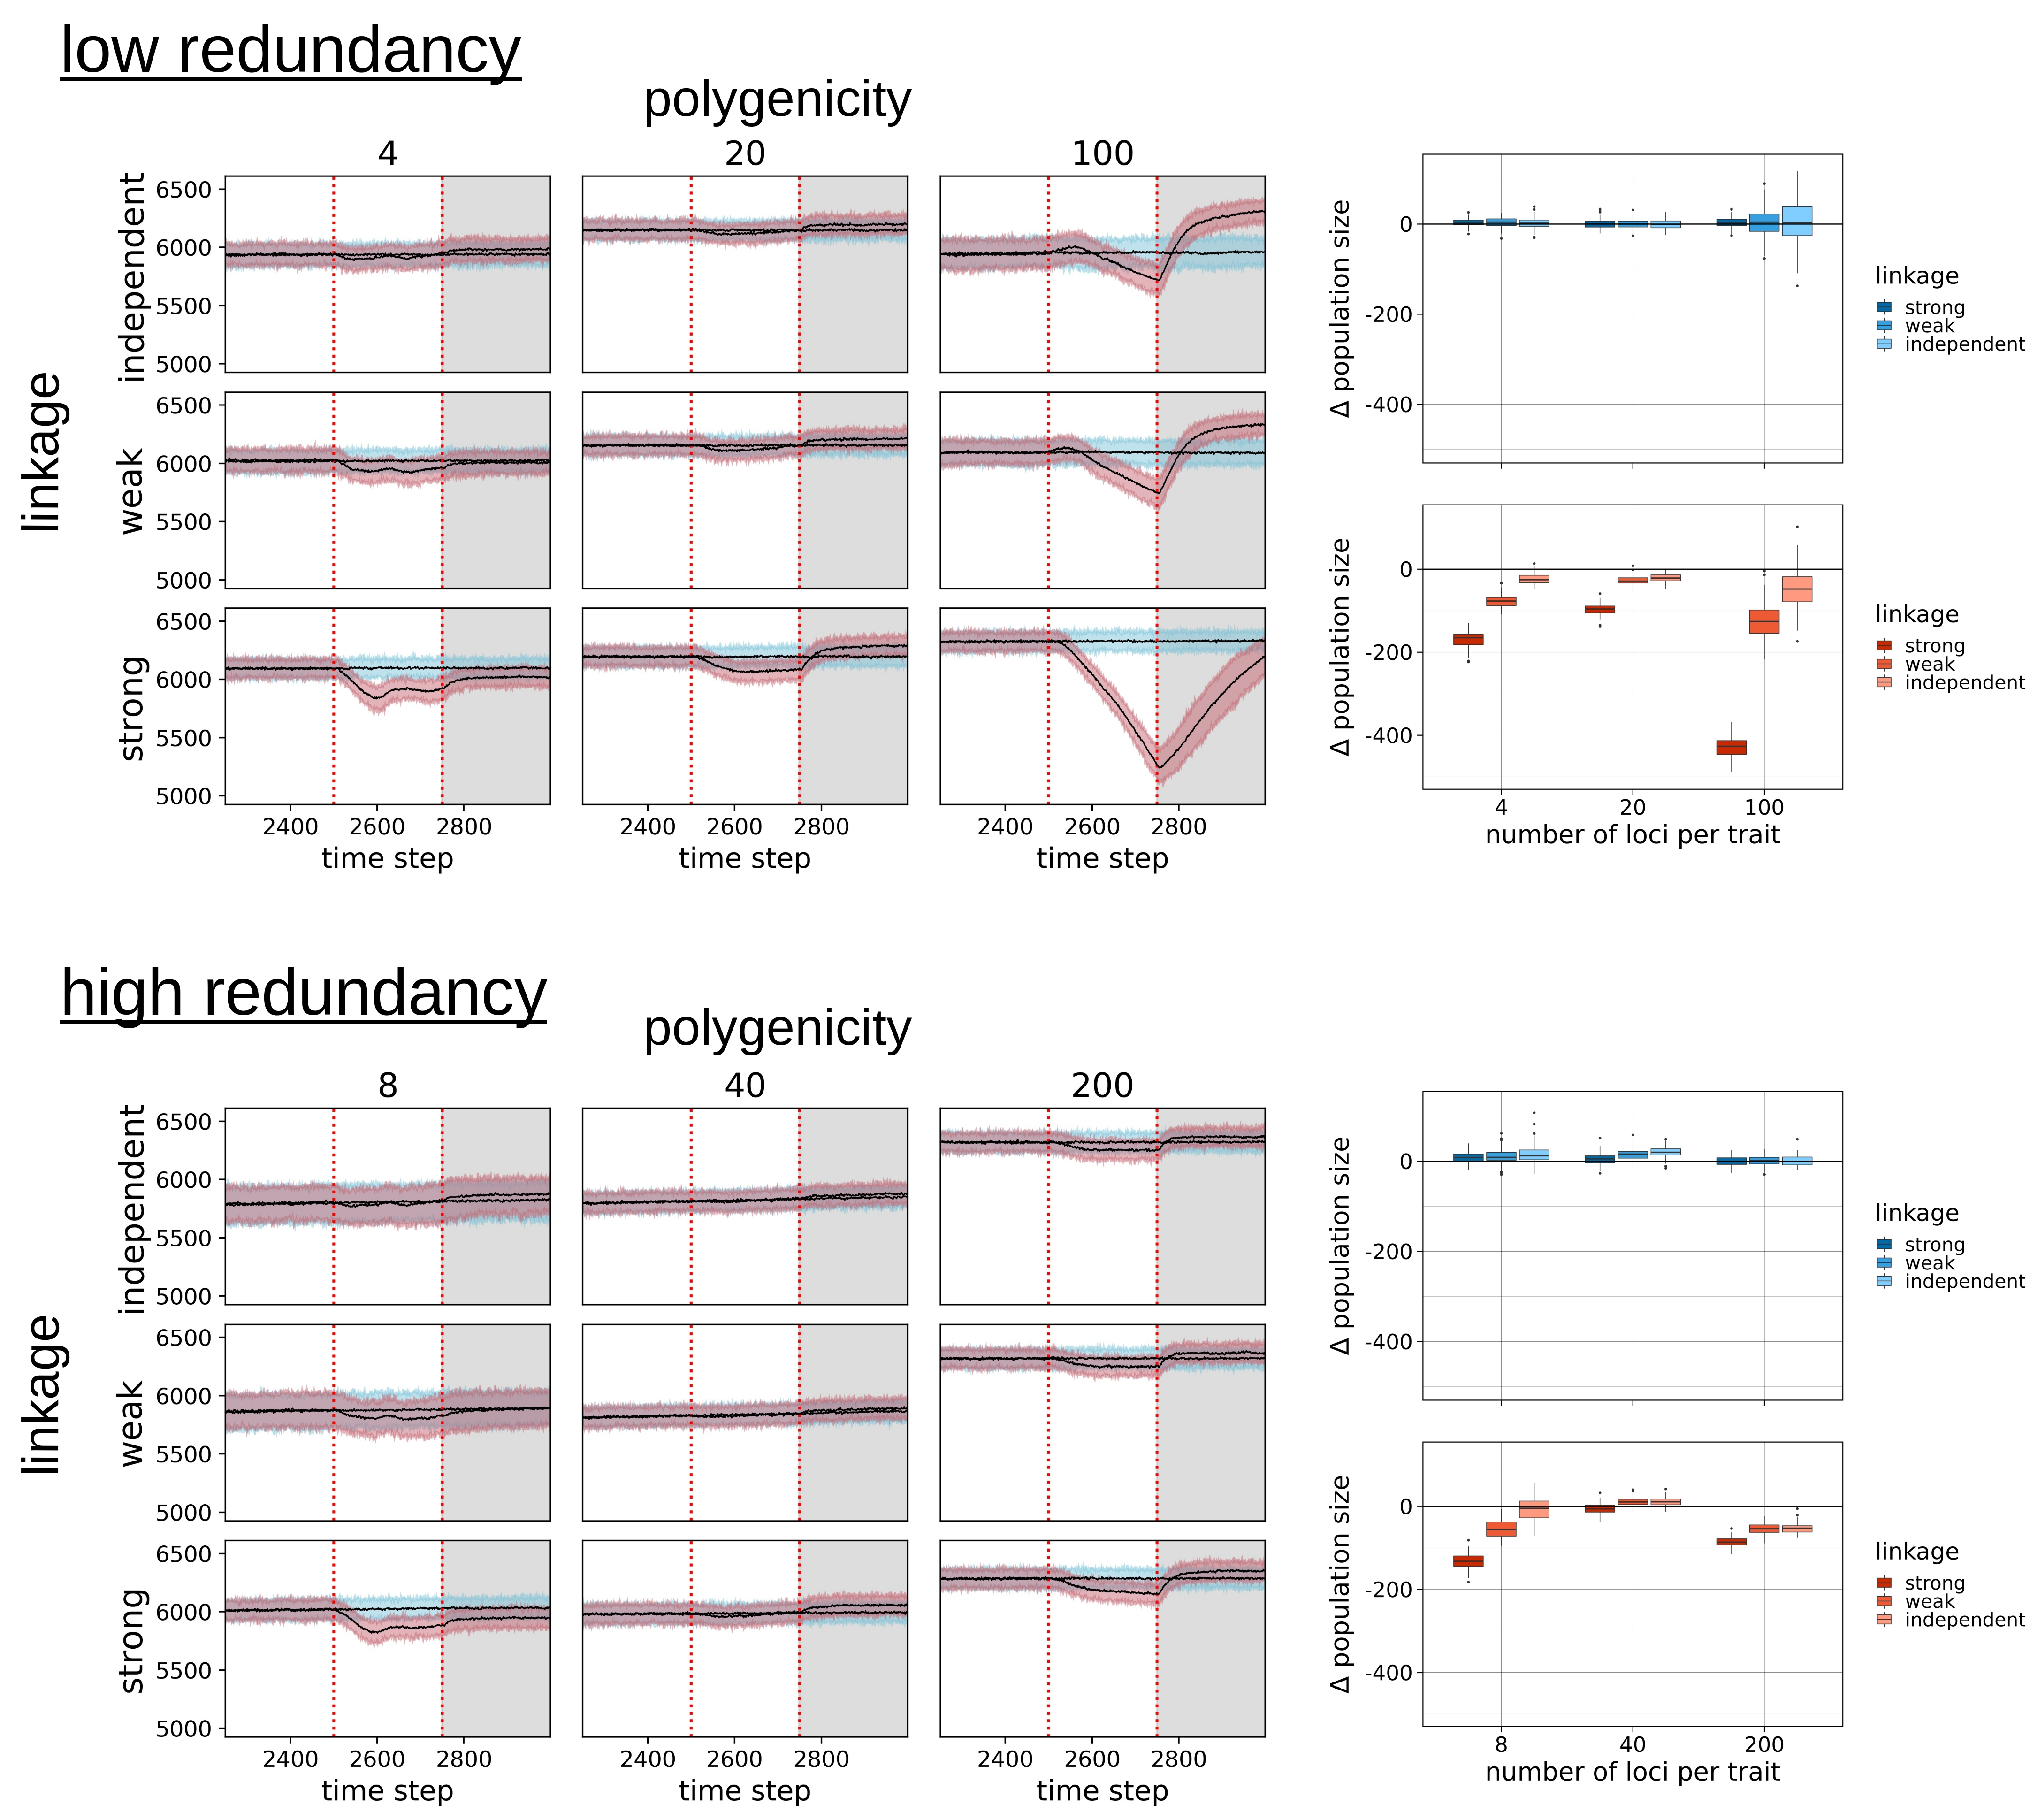
\includegraphics[width=17.8cm]{pub/figs/FIG_S2_Nt_over_time.jpg}
\caption{Left: Population size dynamics for all scenarios during the 250 time steps before the climate change period and the 250 time steps during it (with the two periods divided by a red, dashed vertical line marking the onset of the climate change period). Scenarios are organized as in Fig. \ref{fig:fig_2}: top and bottom sections representing low and high redundancy, with rows in each section representing levels of linkage and columns representing polygenicity. Both means (black lines) and variability envelopes (5th percentile to 95th percentile) are shown, with scenario type depicted by color (main scenarios in red, null scenarios in blue). Right: Comparison of climate change-driven changes in mean population size across scenarios. Null scenarios are plotted on the left in blue, and main scenarios are plotted on the right, in red. Within each plot, scenarios are divided by the number of loci per trait (x-axis) and by the strength of linkage (shade, with darker hues representing stronger linkage). Asterisks above each box indicate level of significance (*=0.1, **=0.05, ***=0.005).}
\label{fig:fig_s2}
\end{figure*}

\begin{figure*}
\centering
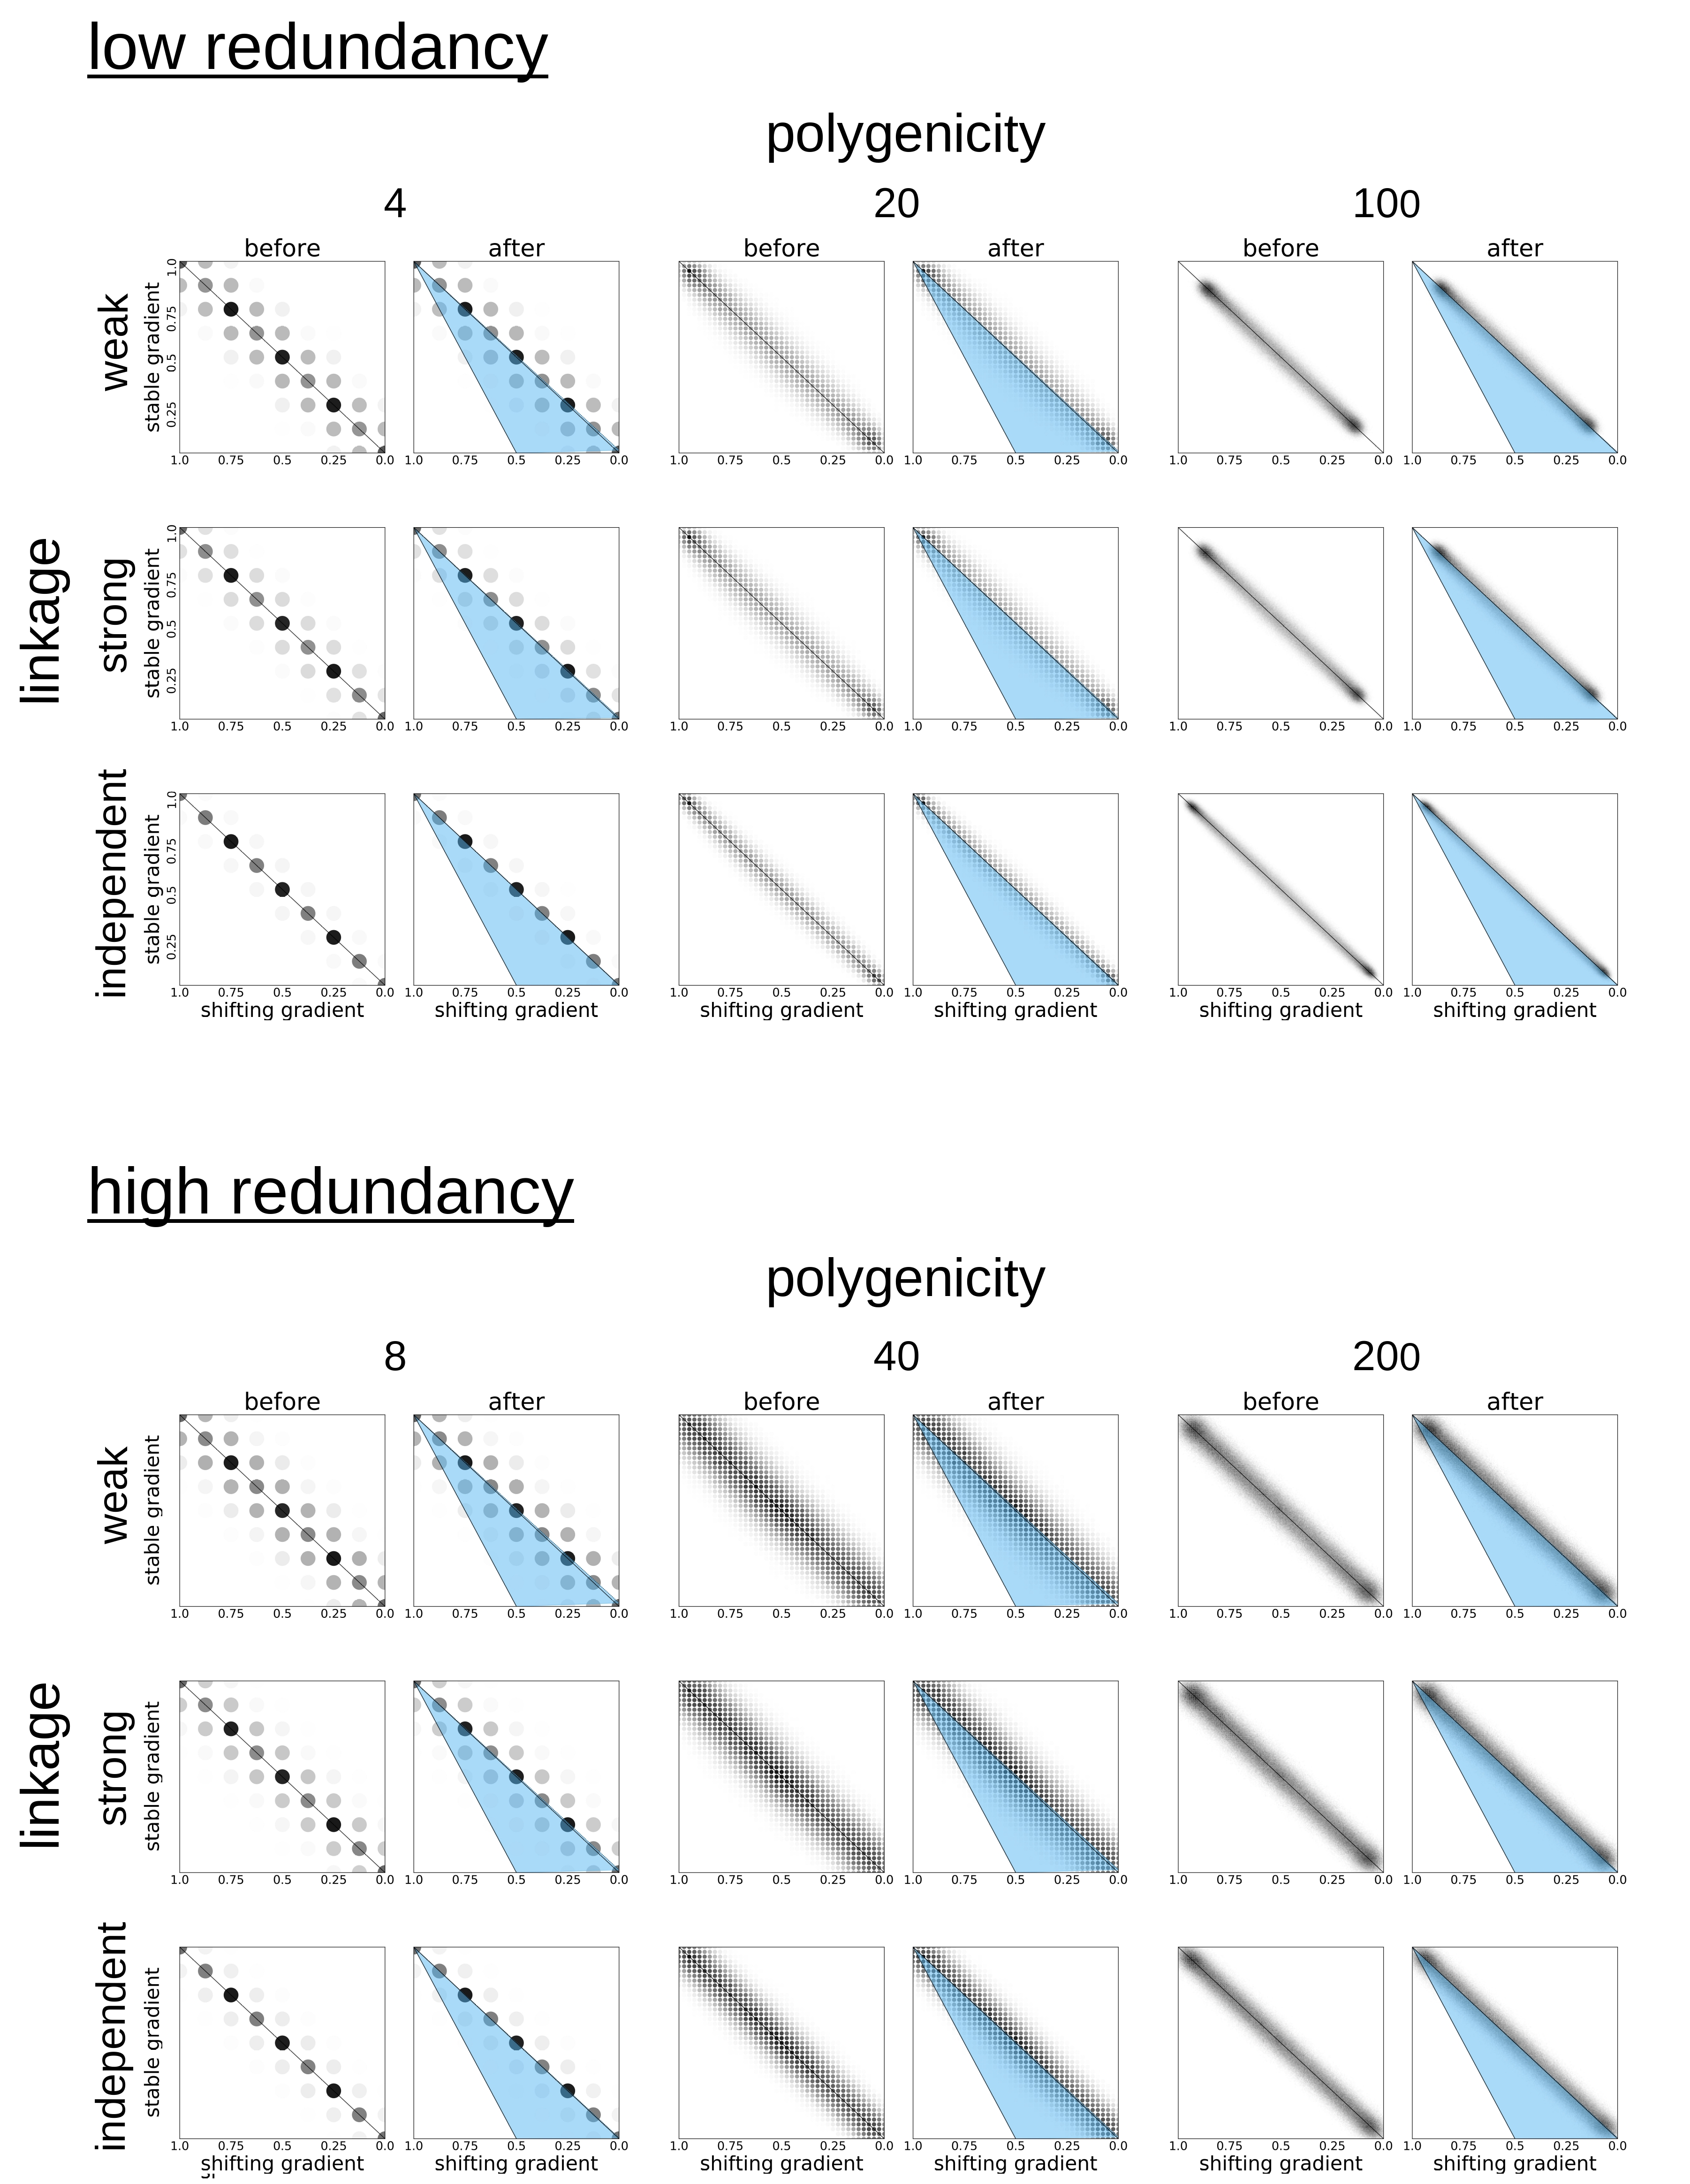
\includegraphics[width=.8\linewidth]{pub/figs/FIG_S3_phenotypic_shift_null.jpg}
    \caption{Maps depicting shifts in population density during climate change for all null simulations. Scenarios are organized as in Fig. \ref{fig:fig_2}: top and bottom sections representing low and high redundancy, with rows in each section representing levels of linkage and columns (in before-after pairs) representing polygenicity. As well as showing local extinction in the low-redundancy, high-polygenicity, strong-linkage scenario (bottom right of top section), these maps also show moderate simulation edge effects and density banding in the low-polygenicity scenarios because of the mismatch between environmental and phenotypic resolutions.}
\label{fig:fig_s3}
\end{figure*}

\begin{figure*}
\centering
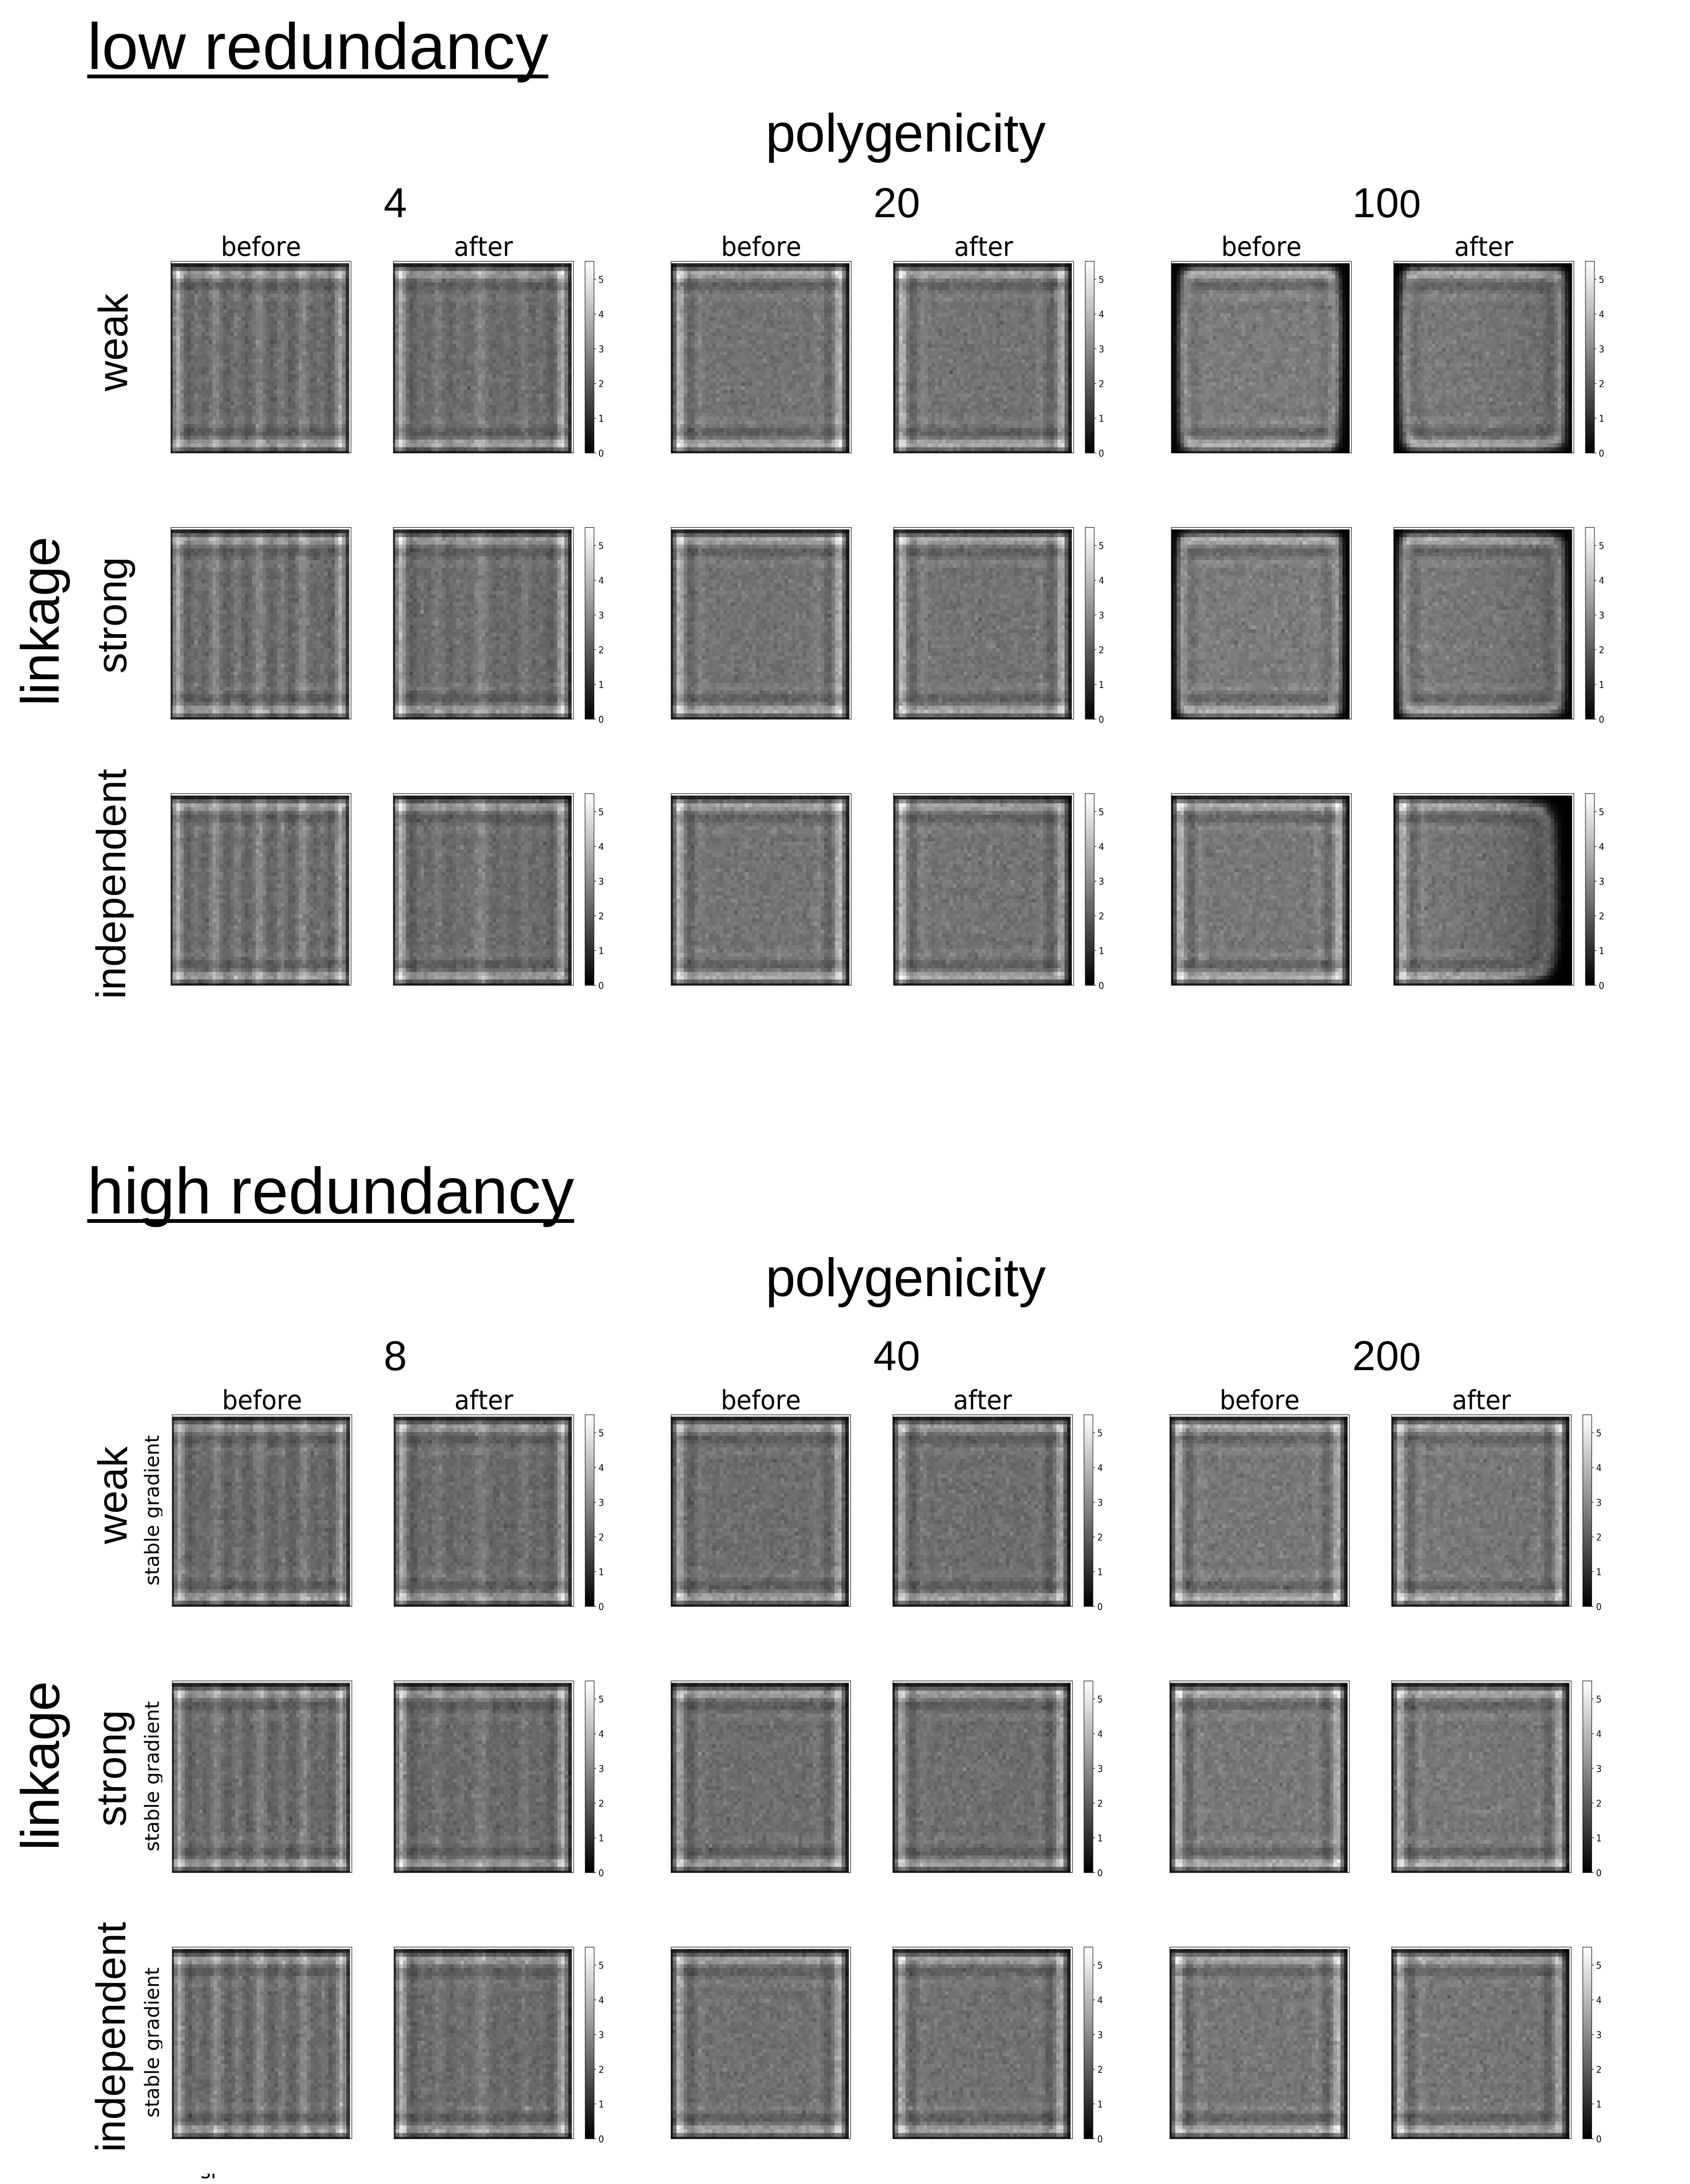
\includegraphics[width=.8\linewidth]{pub/figs/FIG_S4_density_shift.jpg}
\caption{Maps depicting shifts in population density during climate change for all scenarios.}
\label{fig:fig_s4}
\end{figure*}


%%%%%%%%%%%%%%%%%%%%%%%%%%%%%%%%%%%%%%%

\end{document}
